\chapter{Antecedentes}
\label{chap:antecedentes}

\drop{E}{n} este capítulo se introducirán los campos y las tecnologías relacionadas con este
proyecto, realizando una revisión de las mismas. Se realizará un estudio del estado del
arte de los sistemas existentes.

\begin{figure}[h!] 
  \centering
  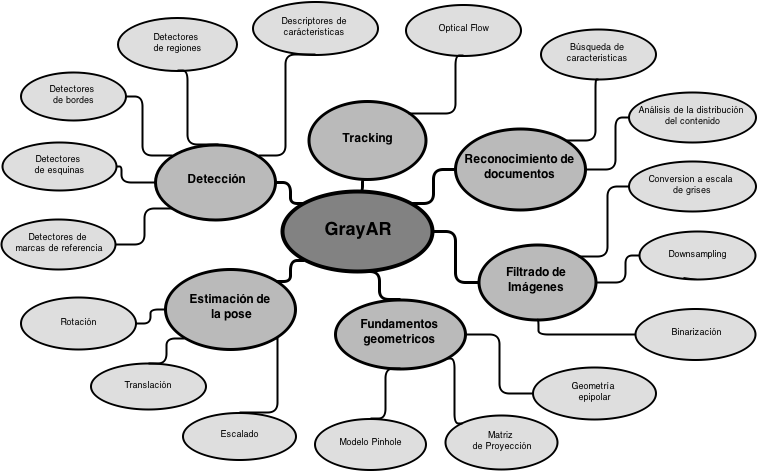
\includegraphics[width=1.0\textwidth]{conceptual_map.png}
  \caption{Antecedentes de GrayAR}
  \label{fig:antecedentes}
\end{figure}


\section{Geometría de la formación de imágenes}
La formación de las imágenes consiste en una representación bidimensional del mundo 3D, perdiéndose la información de profundidad.

La óptica geométrica clásica se basa en modelos de lentes para modelar el proceso de formación de las imágenes. Sin embargo, podemos simplificar este proceso suponiendo que todos los rayos que llegan a la cámara atraviesan un único punto y se proyectan en un plano. Este modelo se conoce como modelo \textbf{\textit{pinhole}}.

Debido a que las lentes no tienen un comportamiento ideal, habrá que añadir al modelo unos parámetros de distorsión que permitan corregirlo y aproximarlo al comportamiento real de la cámara.

\subsection{Estructura del modelo \textit{pinhole}}
El modelo \textbf{\textit{pinhole}} \cite{Hartley} permite modelar el proceso de formación de las imágenes mediante una proyección central, en la cual, de cada punto del espacio tridimensional sale un rayo de luz que pasa por un punto fijo del espacio y intersecta en un plano dando lugar a la imagen.

\begin{figure}[h]
  \centering
  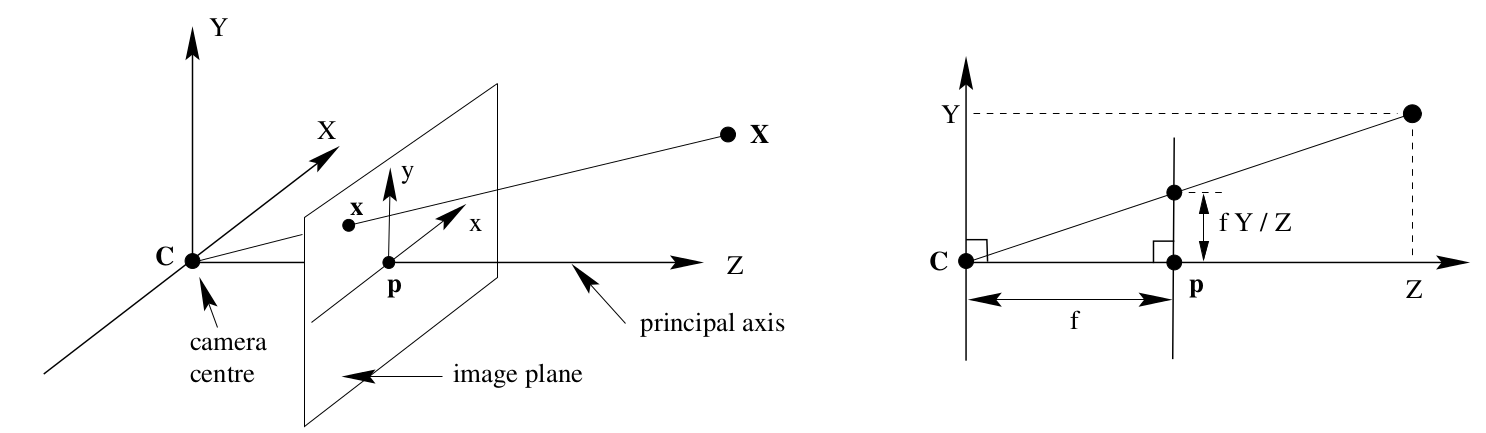
\includegraphics[width=0.85\textwidth]{pinhole.png}
  \caption{Modelo de cámara \textit{pinhole}. La imagen de un punto 3D se forma mediante proyección de perspectiva. Un punto $X$ es proyectado a un punto $x$ en el plano imagen}
  \label{fig:pinholeCamera}
\end{figure}

Los elementos que forman este modelo se definen de la siguiente forma:
\begin{itemize}
\item El \textbf{centro óptico} es el punto fijo del espacio por donde pasan todos los rayos de luz. Se corresponde con el centro de la cámara y es donde se fija el sistema de referencia de la cámara.
\item El \textbf{plano imagen} o plano focal. De cada punto del espacio parte un rayo de luz que pasa por el centro de proyección e intersecta con este plano formando la imagen. Como se puede ver en la figura, el plano focal se ha situado delante del centro óptico. Si éste estuviese detrás, las imágenes estarían invertidas.
\item \textbf{Distancia focal.} Se define como la distancia entre el centro de proyección y el plano imagen.
\item \textbf{Eje principal} Es la línea que pasa por el centro de proyección y es perpendicular al plano imagen.
\item \textbf{Punto principal.} Es el punto de intersección del eje principal con el plano imagen. Coincide con el centro de la imagen.
\item \textbf{Plano principal.} Es el plano paralelo al plano imagen y que contiene al centro de proyección. Además, este plano está formado por todos los puntos cuyas proyecciones se corresponden con puntos en el infinito en la imagen.
\end{itemize}

%Una \textbf{homografía} es una transformación proyectiva que determina una correspondencia entre dos figuras geométricas planas, de forma que a cada uno de los puntos y las rectas de una de ellas le corresponden, respectivamente, un punto y una recta de la otra.

%Una homografía es una matriz (generalmente de 3x3) cuya misión es la de mapear los puntos de una superficie planar bidimensional a otra. Según esta definición, una matriz que transforme los puntos de un plano en puntos del plano de cámara, será considerada una homografía. Esta transformación se realiza en términos de coordenadas físicas.

%\begin{figure}[tb]
%  \begin{minipage}{13.1cm}
%    \centering
%    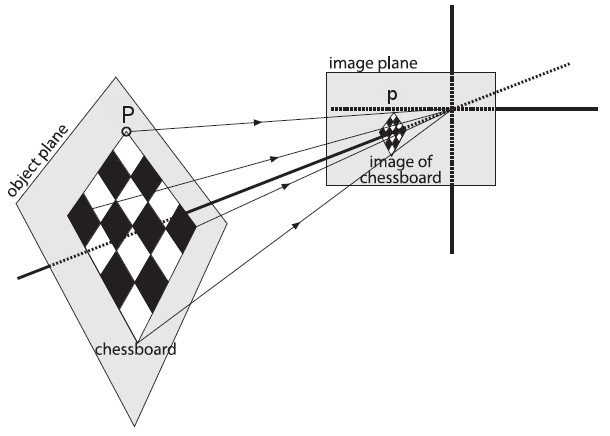
\includegraphics[width=10cm]{homografia.jpg}
%        \cite{OpenCV}.}{}}{}{\caption{Transformación de un punto P del mundo real a su proyección p
%        en el plano de cámara utilizando una homografía. (Bradski y Kaehler)}}
%    \ifthenelse{\equal{FIGhomografia}{}}{}{\label{FIGhomografia}}
%  \end{minipage}
%\end{figure}

%Se ha introducido el parámetro $s$, el cual es un factor de escala arbitrario (entendiéndose que la homografía está definida bajo ese factor, debido al desconocimiento de las medidas del mundo real). En la figura \ref{FIGhomografia} puede verse la implicación de utilizar la homografía en este escenario.

%Podría llegar a pensarse que las funciones de la matriz esencial y de la homografía son las mismas,
%puesto que ambas realizan transformaciones en la geometría del sistema de visión estereoscópica sin tener en cuenta los parámetros intrínsecos de la cámara. La diferencia reside en que la homografía trabaja sobre planos que son visibles desde la cámara y relacionaría un punto de ese plano con el de su propio plano. La matriz esencial no tiene en cuenta esta restricción y solo es capaz de relacionar un punto en una imagen que se encuentre alineado con otra imagen.

\subsection{Matriz de proyección}\label{subsec:matproy}
El modelo \textit{pinhole} \cite{Hartley} fija un sistema de coordenadas proyectivas en el centro óptico. El eje $Z$ de este sistema coincide con el eje principal de la cámara. A partir de ahora nos referiremos a este sistema de coordenadas como sistema de referencia de la cámara. Además, el plano imagen se fija en el plano $Z = f$.

\begin{figure}[h]
  \centering
  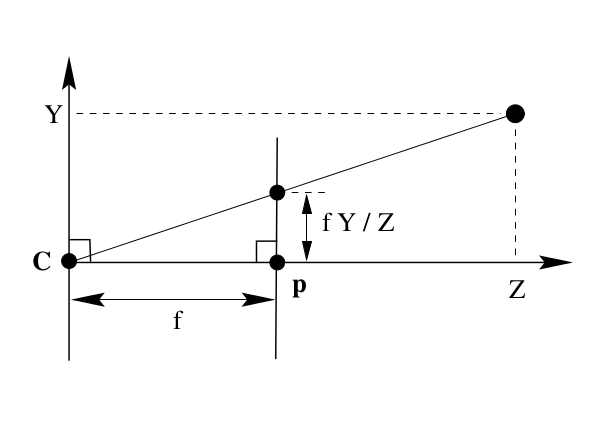
\includegraphics[width=0.8\textwidth]{pinhole2.png}
  \caption{Modelo de cámara \textit{pinhole} visto desde el eje $X$}
  \label{fig:pinholeCamera2}
\end{figure}

Utilizaremos $[X, Y, Z]$, para representar vectores fila. Por tanto, su traspuesta, $[X, Y, Z]^T$, será un vector columna. 

Por convenio con la notación anterior, las coordenadas de un punto cualquiera se van a representar por un vector columna, definiendo los siguiente elementos a considerar:
\begin{itemize}
\item $[X_c , Y_c , Z_c ]^T$ Coordenadas de un punto del espacio tridimensional respecto al sistema de referencia de la cámara.
\item $[X_w , Y_w , Z_w ]^T$ Coordenadas del mismo punto del espacio tridimensional respecto a un sistema de referencia asociado al modelo del objeto. Este nuevo sistema de referencia es distinto al de la cámara.
\item $[x, y]^T$  Coordenadas del punto proyectado en el plano imagen.
\item $f$  Distancia focal
\end{itemize}

Mediante relación de semejanza de triángulos, de la figura \ref{fig:pinholeCamera2}: 
\begin{equation}\label{eq:semejanza}
\dfrac{x}{f} = \dfrac{X}{Z} \quad \quad \quad \quad \dfrac{y}{f} = \dfrac{Y}{Z} 
\end{equation}

podemos determinar la correspondencia entre un punto cualquiera del espacio y su proyección en el plano imagen:
\begin{equation}\label{eq:proyeccion}
  (X_c , Y_c , Z_c )^T \Longrightarrow  (x, y)^T = (f \dfrac{X_c}{Z}, f \dfrac{Y_c}{Z})^T
\end{equation}

Las coordenadas homogéneas son un instrumento empleado para describir un punto en el espacio proyectivo. Consiste en ampliar el plano euclídeo (en el caso bidimensional) al plano proyectivo, es decir, incluirle los puntos impropios o del infinito. De forma que, un punto de dimensiones $(x, y, z)$, se representa por la terna: $(x/w$, $y/w$, $z/w)$ con $w=1$. %Y un punto impropio es aquel donde $w=0$.

Este sistema de coordenadas tiene la particularidad de que permite pasar fácilmente coordenadas de un número de dimensiones a otro. Para ello, almacena las coordenadas con una dimensión adicional, de tal forma que para un espacio de 3D, utilizaríamos 4 coordenadas. El valor de la coordenada adicional indica entre otras cosas, si el punto se encuentra en el infinito, $w=0$, o es un punto cualquiera, $w \neq 0$. En este sistema, si dos coordenadas son proporcionales, se refieren al mismo punto.

Utilizándolas, podemos expresar un punto del espacio tridimensional respecto al sistema de referencia de la cámara de forma matricial:
\begin{equation} 
\begin{pmatrix}
    X_{c} \\
    Y_{c} \\
    Z_{c} \\
    1
  \end{pmatrix}
  \Longrightarrow
  \begin{pmatrix}
    fX_{c} \\
    fY_{c} \\
    Z_{c} \\
  \end{pmatrix}
  =
  \begin{bmatrix} f & 0 & 0 & 0 \\ 0 & f & 0 & 0 \\ 0 & 0 & 1 & 0 \\\end{bmatrix}
  \begin{pmatrix} X_{w} \\  Y_{w} \\  Z_{w} \\  1 \\\end{pmatrix}
\end{equation}
y la expresión de relación de correspondencia, queda de la siguiente forma:
\begin{equation} 
\sigma
\begin{pmatrix}
    X_{w} \\
    Y_{w} \\
    Z_{w} \\
    1
  \end{pmatrix}
=
  \begin{bmatrix} f & 0 & 0 & 0 \\ 0 & f & 0 & 0 \\ 0 & 0 & 1 & 0 \\\end{bmatrix}
  \begin{pmatrix} X_{c} \\  Y_{c} \\  Z_{c} \\  1 \\\end{pmatrix}
\end{equation}

Y de forma abreviada:

\begin{equation}\label{eq:proy}
\sigma \overline{x_w} = P \overline{X_c}   
\end{equation}
donde:
\begin{itemize}
\item $P = diag(f, f, 1) [I|0]$
\item $diag(f, f, 1)$ es una matriz diagonal.
\item $[I|0]$ representa una matriz identidad de 3x3 concatenada con un vector columna nulo de dimensión 3.
\item $\overline{X_c}$  es el vector columna, de dimensión 4, que representa las coordenadas homogéneas del punto del espacio respecto al sistema de referencia de la cámara.
\item $\overline{x}$  es el vector columna, de dimensión 3, que representan las coordenadas homogéneas del punto de la imagen.
\item A la matriz $P$ de se la denomina \textbf{matriz homogénea de proyección de la cámara}.
\end{itemize}


\subsection{Parámetros intrínsecos de la cámara}
La matriz de proyección $P$ de la ecuación \ref{eq:proy} permite transformar las coordenadas de un punto 3D del mundo real en píxeles de una imagen. Se construye a partir de una matriz $K$ y un vector de valores nulos:
\begin{equation}
 P = [K|0] 
\end{equation}
donde la $K$ es la \textbf{matriz de la cámara}, la cuál está formada por una serie de parámetros, denominados \textbf{parámetros intrínsecos}:

\begin{equation}
  K =
  \begin{bmatrix}
    f_{x} & \gamma & {c_{x}} \\
    {0}&{f_{y}}&{c_{y}}\\
    {0}&{0}&{1}
  \end{bmatrix}
\end{equation}

Los \textbf{parámetros intrínsecos} son aquellos que describen las características ópticas y geométricas de una cámara y son constantes. Entre estos parámetros se encuentran la distancia focal, el centro óptico y el punto principal. En la figura \ref{fig:FIGparamCam} se pueden visualizar estos tres parámetros.

\begin{figure}[h]
  \centering
  \includegraphics[width=0.7\textwidth]{parametrosCamara.pdf}
  \caption{Parámetros intrínsecos de una cámara.}
  \label{fig:FIGparamCam}
\end{figure}

\begin{itemize}
\item El \textbf{centro óptico} o centro de proyección, es el punto de la cámara desde el cual parten todos los rayos que son proyectados en el plano de imagen de la cámara.

\item El \textbf{punto principal}, denotado como \textbf{\textit{c}}, es la proyección ortogonal del centro óptico sobre el plano de cámara.  $c_x$, $c_y$ indican el desplazamiento del centro de coordenadas del plano imagen, respecto al punto principal. Será nulo sólo si el eje óptico coincide con el centro del sensor de la cámara, pero el eje óptico no siempre atraviesa el centro de la imagen generada. 

\item El \textbf{factor $\gamma$ (\textit{skew factor})} determina el grado de perpendicularidad de las paredes de los píxeles del sensor. Es inversamente proporcional a la tangente del ángulo que forman los ejes $X$ e $Y$, por lo que  $\gamma$ tendrá un valor nulo si los píxeles son rectangulares. Esto suele ser así en casi todos los sensores utilizados hoy en día. 

\item La \textbf{distancia focal}, es la distancia existente entre el centro óptico y el punto principal. $f_x$ y $f_y$ son dos distancias focales en píxeles. Son proporcionales a la longitud focal $f$ considerada en las ecuaciones (\ref{eq:semejanza}) y (\ref{eq:proyeccion}), según 
\begin{equation}
f_x = f S_x \quad \quad  \quad \quad f_y = f S_y
\end{equation}
donde: $f$ es la longitud focal física de la lente, en unidades de longitud (milímetros, micras, etc.). $S_x$ y $S_y$ son el número de píxeles por unidad de longitud del sensor, a largo del eje $X$ y del eje $Y$ respectívamente. Como es obvio, si el sensor tiene el mismo número de píxeles por unidad de longitud en todas sus dimensiones, las dos focales $f_x$ y $f_y$ tendrán el mismo valor.
\end{itemize}

\subsection{Distorsión}
El uso de lentes facilita la entrada de luz, un enfoque adecuado y una mayor versatilidad, pero también introduce deformaciones en las imágenes que se forman en el sensor. Para el cálculo de coeficientes de distorsión, se tienen en cuenta factores radiales y tangenciales. 

La \textbf{distorsión radial}, consiste en el desplazamiento de los píxeles de de la imagen, de tal modo que las líneas situadas en los extremos del encuadre aparentarán salir hacia el exterior o el interior.   

Para la correción de la distorsión radial de las coordenadas de un pixel de la imagen, se utiliza la siguiente fórmula:
\begin{equation}
  \begin{split}
    x_{corrected} = x(1 + k_1 r^2 + k_2 r^4 + k_3 r^6)  \\
    y_{corrected} = y(1 + k_1 r^2 + k_2 r^4 + k_3 r^6)
  \end{split}
\end{equation}

La textbf{distorsión tangencial} se produce porque la lente no se encuentra perfectamente paralela al plano de imagen. Se puede corregir a través de las siguientes fórmulas:
\begin{equation}
  \begin{split}
    x_{corrected} = x + [ 2p_1xy + p_2(r^2+2x^2)] \\ 
    y_{corrected} = y + [ p_1(r^2+ 2y^2)+ 2p_2xy]
  \end{split}
\end{equation}

%Por otra parte, se obtiene un vector con los factores de distorsión de la cámara. Normalmente este vector contiene 5 valores, correspondientes a 3 factores de distorsión radial, denotados como $k_{i}$ y 2 factores de distorsión tangencial, denotados como $p_{j}$. El número de factores de distorsión radial puede verse incrementado hasta 5, dependiendo del algoritmo de calibración que se realice.
De tal forma que tenemos cinco parámetros de distorsión que son representados en OpenCV como una matriz fila con 5 columnas: 

\begin{equation}
  Distortion_{coefficients} = [k_1 \hspace{10pt} k_2 \hspace{10pt} p_1 \hspace{10pt} p_2 \hspace{10pt} k_3]
\end{equation}

% \begin{figure}[h!]
%   \ifodd\thepage\hspace{-5.2cm}\else\hspace{-0.1cm}\fi\begin{minipage}{13.1cm}
%     \centering
%     \includegraphics[width=9cm]{extrinsicCamara}
%     \ifthenelse{\equal{Transformación geométrica dada por los parámetros extrínsecos entre la posición inicial y final de una cámara. Imagen: \textit{Learning OpenCV} \cite{OpenCV}}{}}{}{\caption{Transformación geométrica dada por los parámetros extrínsecos entre la posición inicial y final de una cámara. Imagen: \textit{Learning OpenCV} \cite{OpenCV}}}
%     \ifthenelse{\equal{FIGextrinsicCam}{}}{}{\label{FIGextrinsicCam}}
%   \end{minipage}
% \end{figure}

\subsection{Parámetros extrínsecos de la cámara}
En la sección \ref{subsec:matproy} se asumió el hecho de que el centro óptico \textbf{C} era el origen de coordenadas del mundo. Esto era así a efectos del cálculo de parámetros intrínsecos, con lo cual el modelo era válido siempre que el sistema no fuera movido de su posición inicial.

Por otro lado, en la mayor parte de las aplicaciones prácticas es necesario que la cámara se mueva o se gire, para captar adecuadamente la escena. Por ello, para poder modelar el sistema con independencia de que su posición haya sido alterada o de que un objeto se pueda referenciar respecto al origen de coordenadas de la cámara, es necesario modificar la ecuación \ref{eq:proy} introduciendo un matriz de transformación $T$ 

\begin{equation}
\sigma x = KTX  
\end{equation}

$W = [R|t]$ donde: R es una matriz de rotación, que representa un giro de la cámara (o de un objeto respecto de ella). Tendrá una forma distinta dependiendo de respecto a que eje (X, Y, Z) se haga la rotación:


%Tanto la matriz de cámara como el vector de distorsión contienen únicamente parámetros intrínsecos, lo que significa que serán constantes. No ocurre lo mismo con los parámetros extrínsecos, que varían en función de la situación de la cámara en el escenario, y que producen una matriz de rotación y un vector de traslación. Estos dos elementos indican la transformación geométrica que hay que realizar sobre la cámara para alcanzar la posición y la rotación finales desde su posición inicial. En la figura \ref{fig:RT} se puede ver gráficamente la implicación de los parámetros extrínsecos.

Los \textbf{parámetros extrínsecos} son aquellos que definen la posición y la orientación de la cámara con respecto al mundo real.

Comúnmente, para la determinación de estos parámetros significa:
\begin{itemize}
\item Encontrar el \textbf{vector de translación} entre las posiciones relativas al origen de dos sistemas de referencia.
\item Encontrar la \textbf{matriz de rotación} que provocan los ejes correspondientes a los dos sistemas de referencia alineados ( ej.: uno sobre otro)
\end{itemize}

\begin{figure}
  \centering
  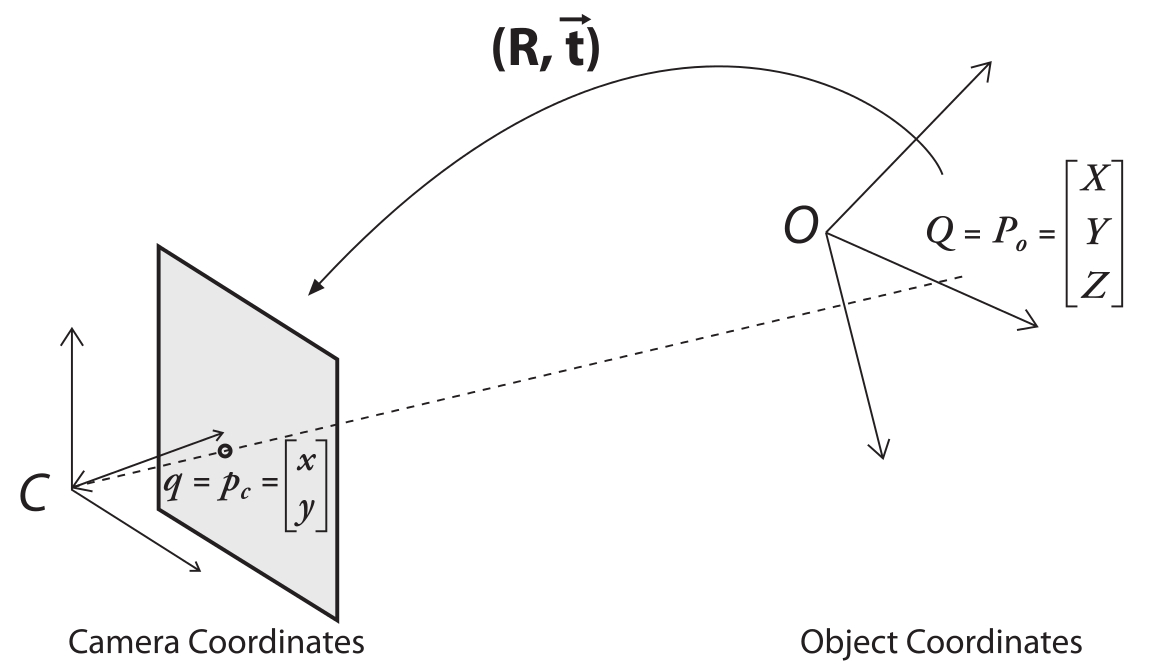
\includegraphics[width=0.8\textwidth]{rt.png}
  \caption{Conversión del sistemas de coordenadas del objeto al sistema de la cámara. El punto $p_c$
    está relacionado con el punto $P_0$ mediante la aplicación de una la matriz de rotación y el
    vector de traslación. (Bradski y Kaehler)}
  \label{fig:RT}
\end{figure}

El proceso de estimación de pose de un objeto consiste en determinar los parámetros de rotación y translación de dicho objeto a partir de información visual. El problema se consolida como uno de los retos más destacados en el campo de la visión por computador, surgiendo numerosas alternativas y métodos para solucionarlo.

La pose del objeto viene determinada por una posición (3 parámetros: X, Y, Z) y una orientación (3 ángulos: yaw, pitch, roll) que forman un conjunto de 6 grados de libertad (6DOF). La solución para la estimación de la pose ha sido propuesta, entre otros métodos, mediante transformada lineal directa (DLT), algoritmos Pnp (perspective-n-point).

%El objetivo es encontrar una correspondencia entre puntos de la imagen en 2D y sus coordenadas en el mundo 3D. A la hora de representar los objetos del espacio observado (3D), los convertimos a un plano de visión (2D), y tenemos que definir cual es la correspondencia entre las coordenadas del espacio y las de la representación. Para facilitar esta conversión, se utiliza el sistema de coordenadas ``homogéneo''. 

Las matrices de transformación, utilizadas para pasar de unas dimensiones a otras, suelen incluir 3
tipos de transformaciones \textbf{R}otación, \textbf{T}ranslación y e\textbf{S}calado. Podemos representarlas así:
\begin{equation}
  [R|t] = \begin{bmatrix} SR_{1,1} & SR_{1,2} & SR_{1,3} & T_{1}  \\
    SR_{2,1} & SR_{2,2} & SR_{2,3} & T_{2}  \\
    SR_{3,1} & SR_{3,2} & SR_{3,3} & T_{3}  \\
    0    &     0   &     0   &  1
  \end{bmatrix}
\end{equation}

%Para convertir las coordenadas del mundo a coordenadas de pantalla, de espacio tridimensional a bidimensional, los sistemas de visión artificial utilizan la siguiente fórmula:
%\begin{equation}
%q=MQ
%\end{equation}
%donde:
%\begin{center}
%$q=\begin{bmatrix} x \\ y \\ z \end{bmatrix}$, $M=\begin{bmatrix} f_{x} & 0 & c_{x} \\ 0 & f_{y} & c_{y} \\ 0 & 0 & 1 \end{bmatrix}$ y %$Q=\begin{bmatrix} X \\ Y \\ Z \end{bmatrix}$
%\end{center}

%Por tanto, $q$ representa el espacio bidimensional en coordenadas homogéneas, y $Q$ el espacio tridimensional. $f_{x}$ es la distancia focal en el eje $X$, $f_{y}$ la distancia focal en el eje $Y$, ($c_{x},c_{y}$) marcan el punto principal, el punto donde el eje de visión corta el plano de visión (normalmente suele estar en el centro de la imagen, o muy cerca)

%Mediante alguna técnica de resolución al problema PnP, se calcula la pose (rotación y traslación) dado un conjunto de puntos de objeto, sus proyecciones en la imagen correspondiente, así como la matriz de cámara y los coeficientes de distorsión. Esta función encuentra una pose que minimiza el error de reproyección, es decir, la suma de los cuadrados de las distancias entre las proyecciones observados y las puntos proyectados
%La matriz de la cámara se corresponde con sus parámetros intrínsecos. Tanto la matriz como el vector de coeficientes de distorsión se obtienen en un proceso previo de calibración de la cámara y se mantienen fijos y conocidos durante todo el proceso.


%usando los parámetros extrínsecos de la cámara, podemos encontrar la relación entre las coordenadas de un punto $P$ en el mundo $(P_w)$ y las coordenadas de la cámara %$\left(P_c\right)$:
%\begin{equation}
%  P_c=R\left(P_w-T\right)where R=\begin{pmatrix}
%    r_{11} & r_{12} & r_{13}\\
%    r_{21} & r_{22} & r_{23}\\
%    r_{31} & r_{32} & r_{33}
%  \end{pmatrix}
%\end{equation}

%Si $P_c=\begin{pmatrix}{X_c} \\ {Y_c} \\ {Z_c} \end{pmatrix}$ Y $P_w=\begin{pmatrix}{X_w} \\ {Y_w} \\ {Z_w} \end{pmatrix}$, entonces
%\begin{equation}
%  \begin{pmatrix} X_{c}\\ Y_{c}\\ z_{c}\end{pmatrix} =\begin{pmatrix}r_{11} & r_{12} & r_{13}\\r_{21} & r_{22} & r_{23}\\r_{31} & r_{32} & r_{33}
%  \end{pmatrix}\begin{pmatrix}X_{w} - T_{x}\\Y_{w} - T_{y}\\Z_{w} - T_{z}\end{pmatrix}
%\end{equation}
%o
%\begin{equation}
%  X_c=R^{T}_1\left(P_w-T\right)\\
%  Y_c=R^{T}_2\left(P_w-T\right)\\
%  Z_c=R^{T}_3\left(P_w-T\right)
%\end{equation}
%donde $R^{T}_i$ corresponde a la fila $i-th$ de la matriz de rotación.



%\begin{figure}[h!]
%  \centering
%  \includegraphics[width=0.6\textwidth]{extrinsicCamara}
%  \caption{Transformación geométrica dada por los parámetros extrínsecos entre la posición inicial y final de una cámara.}
%  \label{fig:FIGextrinsicCam}
%\end{figure}

%\subsection{Combinación de parámetros extrínsecos e intrínsecos de la cámara}

%La matriz que contiene los parámetros intrínsecos de la cámara:
%\begin{equation}
%  M_{in}=\begin{pmatrix}-\frac{f}{s_x} & 0 & 0_{x}\\0 & -\frac{f}{s_y} & o_y\\0 & 0 & 1\end{pmatrix}
%\end{equation}
%- La matriz que contiene los parámetros extrínsecos de la cámara:
%\begin{equation}
% M_{ex}=\begin{pmatrix}r_{11} & r_{12} & r_{13} & -R_1^TT\\r_{21} & r_{22} & r_{23} & -R_2^TT\\r_{31} & r_{32} & r_{33} & -R_3^TT\end{pmatrix}M_{ex}=\begin{pmatrix}r_{11} & r_{12} & r_{13} & -R_1^TT\\r_{21} & r_{22} & r_{23} & -R_2^TT\\r_{31} & r_{32} & r_{33} & -R_3^TT\end{pmatrix}
%\end{equation}

%Usar coordenadas homogéneas:
%\begin{equation}
%  \begin{pmatrix}x_{h}\\y_{h}\\w \end{pmatrix}=M_{in}M_{ex}\begin{pmatrix}x_{w}\\y_{w}\\z_{w}\\1 \end{pmatrix}=M\begin{pmatrix}x_{w}\\y_{w}\\z_{w}\\1 \end{pmatrix}=\begin{pmatrix}m_{11} &m_{12} & m_{13} & m_{14}\\m_{21} & m_{22} & m_{23} & m_{24}\\m_{31} & m_{32} & m_{33} & m_{34}\\m_{41} & m_{42} & m_{43} & m_{44}\end{pmatrix}\begin{pmatrix}x_{w}\\y_{w}\\z_{w}\\1 \end{pmatrix}
%\end{equation}
%
%La homogeneización es necesaria pra obtener las coordenadas píxel:
%\begin{equation}
%  x_{im}=\frac{x_h}{w}=\frac{m_{11}X_w+m_{12}Y_w+m_{13}Z-w+m_{14}}{m_{31}X_w+m_{32}Y_w+m_{33}Z-w+m_{34}}
%  y_{im}=\frac{y_h}{w}=\frac{m_{21}X_w+m_{22}Y_w+m_{23}Z-w+m_{24}}{m_{31}X_w+m_{32}Y_w+m_{33}Z-w+m_{34}}
%\end{equation}

%Llamamos M a la proyección de la matriz (es una matriz 3x4)
%
%Nota: la relación de los puntos 3D y sus proyecciones 2D pueden ser vistas como una transformación lineal de la proyección espacial $({X_w}, {Y_w}, {Z_x}, 1)^T$ a la proyección del plano $({X_h}, {Y_h}, w)^T$.


\subsection{Visión Estereoscópica}

Un proyector se calibra usando los mismos algoritmos de calibración que una cámara ya que puede
considerarse como una ``cámara inversa''. No obstante el hecho de poder aplicar un modelo pin-hole
a un proyector no parece tan evidente como en el caso de una cámara. Para la calibración de un
proyector es inevitable el uso al menos una cámara. Para calibrar un proyector, ya sea usando el
método de Tsai \cite{Tsai}, como el método de Zhang \cite{Zhang99} es necesario obtener un conjunto
de coordenadas 3D-2D correspondientes. La \textbf{Visión Estereoscópica} consiste en el empleo de
dos vistas del mismo espacio desde diferentes puntos de visionado.

\subsubsection{Geometría epipolar}

La geometría más básica en la que se basa cualquier sistema de visión estereoscópica es la \textbf{geometría epipolar}. Se parte de la base de que en un sistema geométrico de este tipo se tienen una cámara izquierda y una cámara derecha.

\begin{figure}
  \centering
  \includegraphics[width=0.7\textwidth]{geometriaEpipolar.pdf}
  \caption{Elementos básicos de la geometría epipolar.}
  \label{fig:FIGgeomEpipolar}
\end{figure}


En la figura \ref{fig:FIGgeomEpipolar} se pueden observar los elementos que componen la geometría
epipolar de un sistema estereoscópico. A cada cámara le corresponde un centro de proyección,
denotados como $O_{l}$ y $O_{r}$, y un plano proyectivo, $\Pi_{l}$ y $\Pi_{r}$. El punto P,
perteneciente al mundo físico tiene una proyección dentro de cada uno de los planos proyectivos. A
estas proyecciones se las denomina como $p_{l}$ y $p_{r}$.


Unos puntos geométricos importantes aquí son los llamados \textbf{epipolos}. Un epipolo $e_l$ (res\-pectivamente $e_r$) en un plano de imagen $\Pi_{l}$ (respectivamente $\Pi_{r}$) se define como la imagen del centro de proyección de la otra cámara $O_{r}$ (respectivamente $O_{l}$). Teniendo presentes estos elementos, existe un plano formado entre el punto P y los dos epipolos $e_{l}$ y $e_{r}$ denominado \textbf{plano epipolar}. Las líneas $p_{l}e_{l}$ y $p_{r}e_{r}$ (líneas que atraviesan los centros de proyección y los correspondientes epipolos), se llaman \textbf{líneas epipolares}.

Para poder entender la utilidad de estos elementos se parte de que el punto P es visto en la cámara de la derecha. Debido a que la cámara solo ve $p_{r}$ (la proyección de P en $\Pi_{r}$), el punto P podría estar localizado en cualquier lugar de la línea definida por $p_{r}$ y $O_{r}$. Obviamente, esta línea contiene P, pero también contiene un gran número de puntos. Lo interesante de esto es que esta línea se encuentra proyectada en el plano de la imagen izquierda $\Pi_{l}$; de hecho, esa proyección es lo que antes ha sido definido como línea epipolar.

Con este escenario, pueden extraerse una serie de propiedades:

\begin{itemize}
\item Todo punto 3D visto por ambas cámaras está contenido en el plano epipolar que intersecta cada imagen en una línea epipolar.
\item Dado un punto 2D en una imagen, su punto asociado en la otra imagen se encuentra a lo largo de la correspondiente línea epipolar. Esto es lo que se conoce como \textbf{restricción epipolar}.
\item La restricción epipolar implica que la búsqueda bidimensional de puntos asociados entre dos vistas se convierte en una búsqueda unidimensional a través de las líneas epipolares una vez conocida la geometría epipolar del sistema estereoscópico.
\end{itemize}


%\subsubsection{Fundamentos matemáticos}

%Una vez conocidos los elementos que describen un sistema estereoscópico, se mostrará la utilización de dos matrices a través de las cuales pueden realizarse transformaciones sobre el sistema estereoscópico. Estas matrices son la \textit{matriz esencial} y la \textit{matriz fundamental}.

\subsubsection{La matriz esencial}

Se define la matriz esencial ($E$) de un sistema estereoscópico como aquella que contiene la información de traslación y rotación que relaciona las dos cámaras en el espacio físico.

Esto significa que, conocidas las coordenadas de un punto $p_{l}$ en la imagen izquierda, puede conocerse su punto correspondiente en la imagen derecha $p_{r}$ multiplicando dicho punto por la matriz esencial del sistema, de tal forma que se cumple la siguiente ecuación:

\begin{equation}
  p_{r}^TEp_{l} = 0
  \label{esencial}
\end{equation}\\
Es importante indicar que la matriz esencial no tiene en cuenta los parámetros intrínsecos de la cámara, por ello es por lo que trabaja en coordenadas físicas.

\subsubsection{La matriz fundamental}

La matriz esencial contiene toda la información acerca de la geometría de una cámara con respecto de la otra, pero no posee información de las cámaras en sí. En la práctica resulta más útil trabajar en unidades de píxel, ya que estas son las que se conocen en primera instancia al trabajar con imágenes.

Para conocer la relación entre un píxel en una imagen y su píxel correspondiente en la otra imagen a través de la linea epipolar debe introducirse información de los parámetros intrínsecos de las cámaras. Para hacer esto, cada punto $p$ se sustituye por $q$, aplicando la matriz de cámara al anterior punto $p$, de tal forma que $q=Mp$, o, de forma equivalente, $p=M^{-1}q$. De esta forma, la ecuación \ref{esencial} se convierte en:

\begin{equation*}
  q_r^T(M_r^{-1})^TEM_l^{-1}q_l=0
\end{equation*}\\
Partiendo de esto, se define la matriz fundamental $F$ como:

\begin{equation}
  F=(M_r^{-1})^TEM_l^{-1}
  \label{defFundamental}
\end{equation}\\
Sustituyendo:

\begin{equation}
  q_r^TFq_l=0
  \label{fundamental}
\end{equation}\\
En esencia, la matriz $F$ es igual que la matriz $E$, excepto que $F$ opera en coordenadas píxel de la imagen, mientras que $E$ trabaja con coordenadas físicas.

Existen un par de propiedades matemáticas interesantes acerca de la matriz fundamental:

\begin{itemize}
\item La matriz $F$ es una matriz de 3x3 que tiene solamente siete grados de libertad, lo que significa que, de los nueve componentes de la matriz, dos pueden ser calculados a partir de los otros siete.
\item El rango de la matriz $F$ es 2.
\end{itemize}

Además de estas propiedades, existen otras propiedades geométricas:

\begin{itemize}
\item Dada una geometría bifocal, la matriz $F$ es función exclusiva de dicha geometría, es decir, es independiente de todos los puntos P de la escena y de las proyecciones $p_l$ y $p_r$ de los puntos de la escena.
\item La matriz $F$ define las líneas epipolares a través de las ecuaciones:

  \begin{equation}
    l_r=Fm_l
  \end{equation}
  \begin{equation}
    l_l=F^Tm_r
  \end{equation}

\item La matriz $F$ define los epipolos a través de las ecuaciones:

  \begin{equation}
    Fe_l=
    \begin{bmatrix}
      0 \\ 0 \\ 0
    \end{bmatrix}
  \end{equation}
  \begin{equation}
    F^Te_r=
    \begin{bmatrix}
      0 \\ 0 \\ 0
    \end{bmatrix}
  \end{equation}

\end{itemize}




\section{Realidad Aumentada}
La realidad aumentada es una tecnología mediante la cual la percepción del mundo real se complementa con información adicional generada por ordenador en tiempo real. Esta información adicional puede ser desde etiquetas virtuales, representaciones de modelos tridimensionales, o incluso cambios de iluminación. 


La Realidad Aumentada es un conjunto de técnicas que permiten integrar en tiempo real contenido digital a la percepción del mundo real.

Según la taxonomía descrita por Milgram y Kishino [16], los entornos
de Realidad Mixta son aquellos en los que “se presentan objetos del
mundo real y objetos virtuales de forma conjunta en una única pan-
talla”. Esto abre un abanico de definiciones en la que se sitúan las
aplicaciones de Realidad Aumentada (ver Figura 1.2).


El término Realidad Aumentada fue acuñado en 1990 por Tom Caudell durante el desarrollo de un sistema de Boeing para ayudar a los trabajadores en el ensamblaje de aviones mediante la ayuda de pantallas que mostraban información del montaje. 

%La realidad aumentada se puede aplicar a prácticamente todos los campos. En el sector industrial, para la reparación y mantenimiento de maquinas e instalaciones complejas, visualización de datos o simulación.  En aplicaciones médicas, mostrarían la situación de órganos no visibles durante una cirugía. También se han realizado aplicaciones para diseño de interiores (IKEA), presentaciones de productos, educación, publicidad, turismo, arte y ocio. 

Uno de los principales problemas a resolver es denominado registro. Los objetos del mundo real y virtual deben estar correctamente alineados o la sensación de integración se verá seriamente afectada. Sin un registro preciso, la realidad aumentada no podría ser soportada por muchas aplicaciones, por ejemplo, en medicina para el guiado de una aguja en la realización de una biopsia. 

Las aplicaciones de Realidad Aumentada deben cumplir las siguientes características definidas por Ronald T. Azuma \cite{Azuma}:
\begin{itemize}
\item \textbf{Combinar el mundo real con el virtual.} El resultado final debe mostrar la información sintética sobre las imágenes percibidas del mundo real.
\item \textbf{Debe ser interactivo en tiempo real.} La integración debe ser realizada \emph{en el momento}, por lo que el cálculo necesario debe realizarse n el menor tiempo posible.
\item \textbf{La alineación de los elementos virtuales debe realizarse en 3D.} Los objetos sintéticos deben de estar en el espacio tridimensional.
\end{itemize}

%\subsection{Componentes de un sistema de realidad aumentada}
%Un sistema de realidad aumentada depende de cuatro componentes físicos:

%\begin{itemize}
%\item \textbf{Elementos de entrada y sensores de orientación.} Proporciona al sistema la información visual, la entrada del usuario y, potencialmente, ayudar a la orientación.
%\item \textbf{Fuente de datos.} Proporciona información aplicable al medio ambiente para que el sistema aumente la visión del usuario.
%\item \textbf{Periféricos de retroalimentación de los usuarios.} Principalmente en la forma de producción visual, pero también pueden incluir audio y otras interfaces de usuario.
%\item \textbf{Unidad de procesamiento.} Combina los datos de los sensores de entrada para determinar la orientación y aumentar la visión del usuario con información de la fuente de datos. Envía el resultado a los periféricos de retroalimentación del usuario.
%\end{itemize}

\subsection{Elementos de entrada y sensores de orientación}
Un sistema de realidad aumentada debe ser capaz de conocer su orientación y posición dentro del entorno circundante con el fin de ofrecer una experiencia «aumentada» satisfactoria. La combinación de la orientación y la posición de un observador que se conoce como \emph{pose}. La estimación de la \emph{pose} se definirá con más detalle en la sección 4. La orientación y posición se pueden determinar mediante técnicas de visión por computador, pero hay métodos alternativos para estimar la \emph{pose}  utilizando  sensores diseñados específicamente para medir alguno o todos los parámetros de los seis grados de libertad que componen la \emph{pose}.

\subsubsection{Localización}
La manera más popular para determinar la posición es mediante la utilización del Sistema de Posicionamiento Global (GPS), desarrollado por el ejército de Estados Unidos y totalmente operativo desde 1994. 
Un receptor GPS es lo suficientemente preciso para determinar la ubicación en las aplicaciones de realidad aumentada, además, debido a su bajo coste, los sensores de GPS se llevan incluido en los teléfonos móviles desde 2005.

\subsubsection{Orientación}
En el espacio 3D, la orientación de un cuerpo rígido puede ser determinado de forma única por tres ángulos o grados de libertad (3DOF): \emph{pitch, roll y yaw}. La figura \ref{fig:ángulos}  se puede observar una representación de estos tres ángulos como rotaciones alrededor de sus ejes correspondientes. 

\begin{figure}[b]
  \centering
  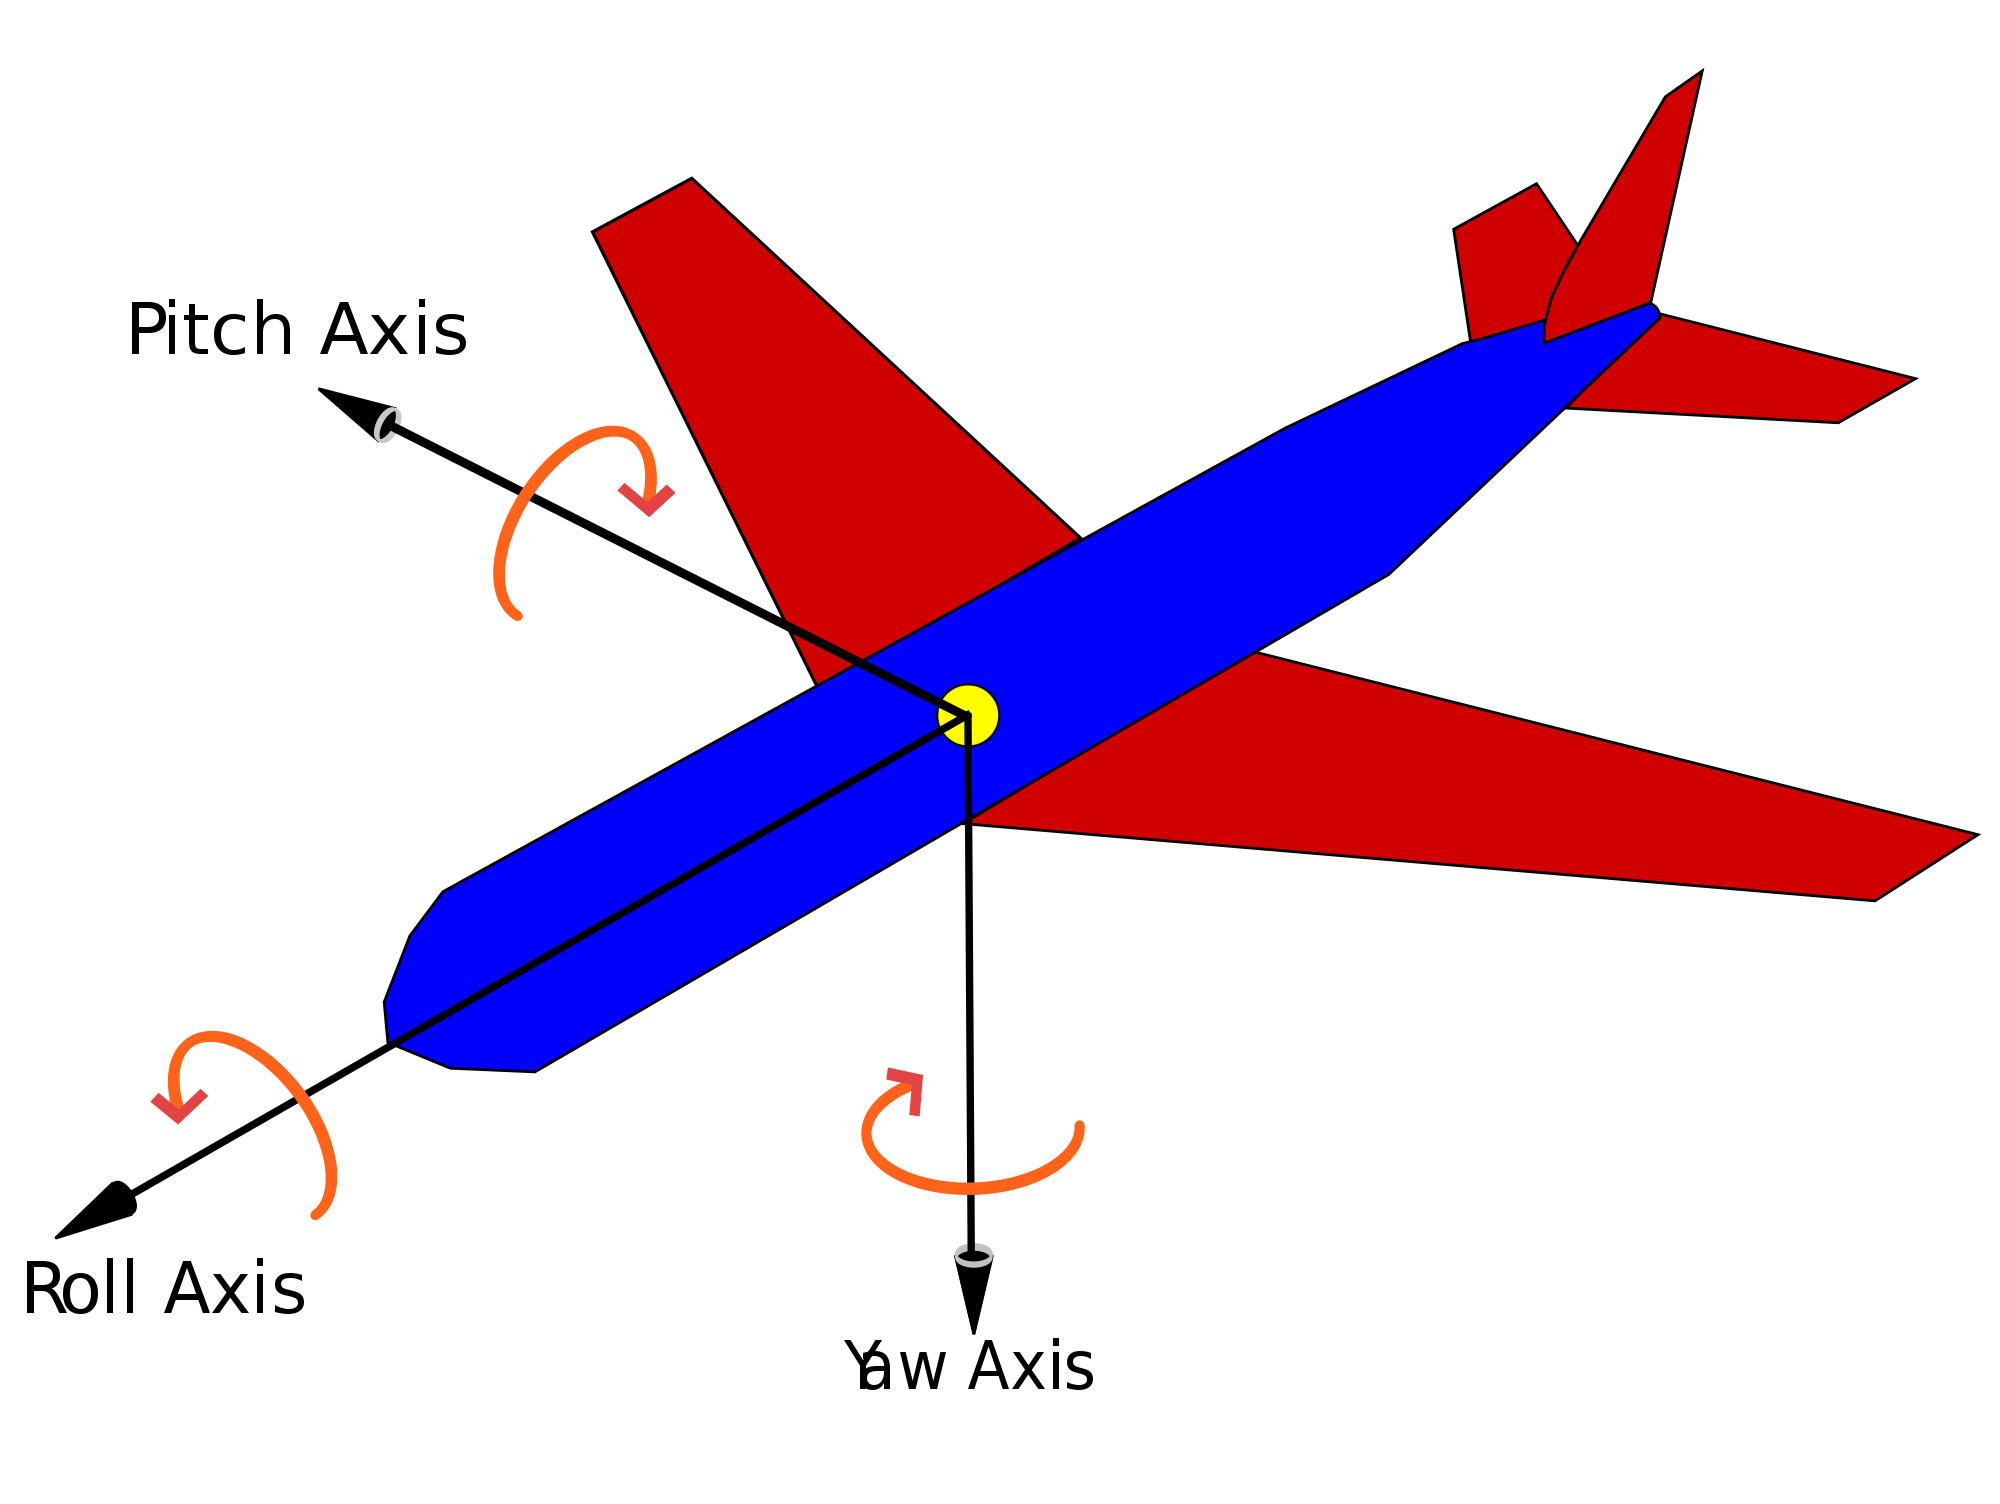
\includegraphics[width=0.5\textwidth]{angles.png}
  \caption{Ángulos de orientación: \emph{yaw, pitch y roll}}
  \label{fig:ángulos}
\end{figure}

Para facilitar la tarea de orientación los dispositivos móviles, sobre todo smartphones y tablets, están equipados una serie de sensores como:

\begin{itemize}
\item\textbf{Sensores magneto-resistivos}, o magnetómetros, que son utilizados como una ``brújula electrónica'' y se utilizan para determinar el \emph{yaw} y la dirección. Las nuevas generaciones de brújulas electrónicas utilizan tres ejes para asegurar una lectura correcta sin importar la inclinación del sensor.
\item\textbf{Acelerómetros} para medir la aceleración aceleración experimentada por un objeto con respecto a un marco de referencia. Los acelerómetros no pueden determinar el \emph{yaw}, pero pueden ser utilizados para determinar el \emph{pitch} y el \emph{roll}. 
\item\textbf{Giroscopios electrónicos} que son utilizados para determinar los tres grados de libertad de orientación a la vez.
\end{itemize}

Un problema común en los sistemas de seguimiento visual es que los movimientos bruscos de la cámara pueden ocasionar que la imagen salga borrosa y verse afectado el seguimiento visual. Un dispositivo híbrido equipado con un giroscopio y un acelerómetro será capaz de determinar rápidamente y con precisión tres de los seis grados de libertad de la \emph{pose} y ayudar al sistema de seguimiento visual a recuperarse cuando se experimentan imágenes borrosas. 

\subsubsection{Fuentes de Vídeo}
La realidad aumentada superpone información sobre lo que el usuario está viendo. Para los sistemas dinámicos en los que la información virtual debe ser mezclada con la imagen real, se requiere un dispositivo de captura, como una cámara digital. Para los propósitos de las aplicaciones de realidad aumentada es preferible una cámara de vídeo. La mayoría de las aplicaciones utilizan una única cámara y se conocen como sistemas monoculares. También existen sistemas estereoscópicos, que  utilizan dos cámaras para determinar la profundidad.

El desarrollo tecnológico en el ámbito de la captura de imagen digital que han mantenido los principales fabricantes en los últimos 10 años, conocido como la «batalla del mega-píxel», ha supuesto un gran avance para disponer de sensores con una gran calidad de imagen y un coste reducido. Actualmente es normal encontrar cámaras de alta resolución en prácticamente todos los dispositivos móviles, permitiendo grabar vídeo en una resolución FullHD ó 4K y obtener imágenes fijas de hasta 7136x5360px.

\subsubsection{Entrada táctil}
En sistemas de realidad aumentada portátiles tales como teléfonos inteligentes o tablets, la pantalla funciona al mismo tiempo como una entrada para manipular objetos directamente en la pantalla y un dispositivo de salida.

\subsection{Fuente de datos}
Un sistema de realidad aumentada requiere una fuente de datos e información con la que aumentar la realidad de un usuario. La fuente de datos puede ser desde una base de datos directamente disponible en el sistema, o puede ser información agregada a partir de fuentes disponibles a través de una conexión de red. Actualmente existe un gran desarrollo para el uso de Internet como fuente de datos para aplicaciones de realidad aumentada. Aplicaciones como Wikitude\footnote{http://www.wikitude.com} y Layar\footnote{http://www.layar.com} son ejemplos de las sistemas que utilizan los datos disponibles en Internet como fuente de datos.

\subsection{Periféricos de retroalimentación de los usuarios}
\subsubsection{Dispositivos  de Visualización}
Existen  muchos métodos y dispositivos para mostrar la información o imágenes generadas para su combinación y alineación con la realidad: 
\begin{itemize}
\item \textbf{Monitores y pantallas tradicionales}
  Sobre todo impulsado por la popularidad de frameworks y bibliotecas como ARToolkit \cite{Kato}, existen muchas implementaciones de realidad aumentada para utilizar con un ordenador de sobremesa o portátil. No requieren de tecnología especial, únicamente una webcam que el usuario puede controlar. La aplicación se suele presentar en una pagina web y permite a los usuarios superponer información o imágenes sobre lo capturado por la webcam. Para la tarea de tracking y registro se utilizan marcadores que el usuario previamente ha impreso.
  
\item \textbf{HMDs (Head Mount Display)} Los HDM o Head Mount Display son dispositivos que permiten al usuario ver el el mundo real con objetos virtuales superpuesto mediante técnicas ópticas y de vídeo. Los HDM se pueden clasificar en dos categorías:
  \begin{itemize}
  \item \textbf{Ópticos (OST - Optical See-Throug)} Permiten al usuario ver el mundo real a través de sus ojos y la imagen virtual se muestra mediante elementos ópticos holográficos, espejos semi-plateados o alguna otra técnica similar. Un ejemplo de este tipo de dispositivo son las Google Glass.
    
  \item \textbf{Vídeo (VST - Vídeo See-Throug)} En los dispositivos de esta categoría, el usuario percibe tanto el mundo real como la imagen virtual mediante una o varias pantallas. Como ventajas de los VST esta una mayor consistencia entre el mundo real y el virtual.
  \end{itemize}
  
\item \textbf{Visualización basada en proyección}
  Un sistema de visualización basado en proyección es una buena opción para sistemas fijos, además proporciona una intrusión mínima y la capacidad de interacción con varios usuarios.
  Se han propuesto una gran variedad de técnicas de visualización mediante proyectores sobre objetos y otras superficies (no necesariamente pantallas). Ehnes \cite{Ehnes} amplió el trabajo anterior de Pinhanez \cite{Pinhanez} sobre la proyección de vídeo para mostrar imágenes virtuales sobre objetos reales directamente utilizando técnicas de tracking de vídeo para seguir el movimiento y manteniendo la imagen sobre objeto mientras este se mueve.
  
\item \textbf{Dispositivos portátiles (smartphones, tablets)}
  Hoy en día el dispositivo portátil por excelencia es el smartphone. Es mínimamente invasivo, muy portable y ampliamente extendido. Según el informe de comScore \footnote{http://www.comscore.com/esl/Insights/Presentations-and-Whitepapers/2013/2013-Spain-Digital-Future-in-Focus} el 66\% de los españoles tienen un teléfono inteligente, por lo que son una gran alternativa para la visualización de aplicaciones de realidad aumentada.
\end{itemize}

\subsubsection{Audio}
El audio se utiliza principalmente de dos formas diferentes en los sistemas de realidad aumentada: como una modalidad de la interfaz de usuario multimodal o para ofrecer una experiencia aural aumentada. 

Por ejemplo, el usuario pueda ser capaz de dar comandos de voz y el sistema devuelva retroalimentación con señales de audio (pitidos). Este tipo de audio no direccional es trivial desde el punto de vista tecnológico aportando una nueva dimensión a las aplicaciones móviles. El audio aumentado puede servir a personas con discapacidad visual para ayudar a comprender el entorno. Mediante unos altavoces o un par de auriculares, es bastante simple proporcionar al usuario la información en forma de audio. La síntesis de voz también se puede utilizar para leer información, por ejemplo, leer palabras en voz alta desde un sistema de reconocimiento de texto.

\subsection{Unidad de procesamiento}
%\subsubsection{Dispositivos móviles: Smartphones,  tablets y SBCs (Single Board Computer)}
El teléfono móvil ha evolucionado hacia una plataforma informática móvil (smartphone), en la que desarrollar las actividades habituales de un ordenador personal. El principal inconveniente de estos era la pantalla reducida que disponen lo que ha derivado en el desarrollo de un nuevo dispositivo denominado tablet. 

Las tablets disponen de prácticamente las mismas características que los smartphones (incluso el mismo sistema operativo) pero las pantallas son mayores, sin necesidad de teclado físico ni ratón, con las que se interactúa principalmente mediante la pantalla táctil con los dedos o un stylus.

Otra tendencia tecnológica es el desarrollo de SBCs, \textit{(Single Board Computer)} que básicamente es un ordenador completo montado sobre un circuito. Su diseño se basa en un microprocesador de bajo rendimiento (normalmente de arquitectura ARM), RAM y diversos dispositivos de E/S como puertos USB, lectores de tarjetas, conectores Ethernet, y salida de audio y vídeo con un precio final muy reducido. Este tipo de dispositivos se crearon para utilizarlos con fines educativos, pero entre la comunidad de usuarios, debido a su gran versatilidad se utilizan para múltiples aplicaciones tales como centros multimedia o distintos tipos de servidores dado su bajo consumo.  

\section{Técnicas de Visión por Computador}
En esta sección comentaremos las técnicas que pueden utilizarse para el tratamiento previo de imágenes que se utilizarán para la detección y tracking en sistemas de realidad aumentada. El orden en que se introducen suele ser el aplicado  habitualmente.

La adquisición de imágenes es el primer paso en un sistema de realidad aumentada y es dependiente de la plataforma del sistema. Por norma general, se considera que las imágenes se adquieren con 24 bits, un canal por cada una de sus componentes de color en 8 bits: rojo, verde y azul. También vamos a asumir que las imágenes se adquieren a 30 fotogramas por segundo. Esta suposición esta basada en la transmisión típica con la que trabajan la mayoría de webcams.

\subsection{Preprocesado de las imágenes de entrada}
Prácticamente todas las técnicas presentadas procesan y trabajan las imágenes en blanco y negro. Aún realizando la captura en color, normalmente se realizan varios pasos previos para reducir y simplificar la cantidad de información que se tiene que manejar, dejando solo la información esencial.

Por ejemplo, un frame típico obtenido a partir de una webcam o la cámara de un teléfono móvil puede tener una anchura de 640 píxeles y 480 píxeles de altura. Suponiendo que una imagen en color con tres canales (rojo, verde y azul) se obtiene con ocho bits por canal, la cantidad de datos por frame serian 640 x 480 x 3 x 8 = 7.372.800 bits de información. Esto es para una sola imagen. La mayoría de cámaras tienen una tasa de transferencia entre 20 y 30 frames por segundo, lo que significa que para cada frame se debe procesar toda esa información por completo cada 33 milisegundos antes de que llegue el siguiente fotograma. Sería muy costoso (e innecesario), por lo que se utilizan una serie de técnicas como las explicadas a continuación para reducir la cantidad de información requerida en las etapas posteriores.

\subsubsection{Conversión a escala de grises}
La reducción del número de canales de la imagen (rojo, verde y azul) a un solo canal de ocho bits representados como gris, reduce la cantidad de datos a procesar en un factor de tres. Una imagen en escala de grises representa la intensidad de la imagen. 

No existe un único método para convertir una imagen en color a escala de grises, el proceso más común consiste en recorrer todos los píxeles de la imagen, y para cada píxel de forma individual multiplicar sus componente RGB (rojo, verde y azul), cuyos valores oscilan entre 0 y 255, por unos coeficientes y sumarlos. De esta forma obtenemos la misma luminosidad del píxel tanto en color como en escala de grises.

Los componentes RGB originales del píxel se sustituyen por el valor resultante de esa suma. Los tres componentes con el mismo valor, para lograr así el efecto de escala de grises, ya que cuando los tres componentes tienen un mismo valor lo que se obtiene es un tono gris, excepto en los extremos, donde (0, 0, 0) es negro y (255, 255, 255) es blanco.

Los coeficientes que se utilizan son 0.299 para el rojo (R), 0.587 para el verde (G), y 0.114 para el azul (B). Al sumar los tres coeficientes el total vale 1 (0.299 + 0.587 + 0.114), lo que garantiza que el valor resultante de la suma de los productos por los componentes originales del píxel será un valor comprendido también entre 0 y 255.

\subsubsection{Thresholding (umbralización o binarización)}
La umbralización consiste en definir un valor umbral y compararlo con cada uno de los píxeles de la imagen. A los píxeles que estén por debajo del umbral se les asigna un valor, y a los que estén por encima otro. De esta forma se divide toda la población de valores en tan sólo dos grupos, reduciendo considerablemente la complejidad de la información a analizar.

Aplicar un valor umbral a una imagen presenta dos dificultades. La primera es decidir que valor concreto tomar, y la segunda es conseguir que dicho valor sirva para cualquier imagen posible que pueda llegar desde la webcam. Si los píxeles tienen un valor que se encuentra dentro del rango que va de 0 a 255, ¿cúal es el mejor valor para el umbral? ¿128, que está en la mitad del rango? ¿Y por qué no 57? No se puede decidir de antemano sin analizar antes la imagen, ya que el mayor inconveniente que presenta este procedimiento es que es muy sensible a la iluminación. Con poca iluminación los píxeles tienden a tomar valores bajos, oscuros, cercanos al 0, y con mucha iluminación toman valores altos, claros, cercanos al 255. Y peor es el caso cuando la iluminación varía dentro de la propia imagen, con algunas zonas muy oscuras y otras muy claras.

El algoritmo de umbralización adaptativa, no aplica el umbral de una manera global sobre todos los píxeles de la imagen, sino que tiene en cuenta las variaciones en la iluminación de una manera local para cada píxel de forma individual. Algo que consigue tomando el valor original de cada píxel de la imagen en escala de grises, y comparándolo con otro valor calculado que sea algún tipo de media de los valores de los píxeles que tiene alrededor. En las zonas homogéneas el valor del píxel se asemejará mucho a la de la media de sus vecinos, mientras que en las zonas de transición abruptas, en los bordes, se diferenciará de dicha media.

La función utiliza un filtro gaussiano para calcular los valores medios de los píxeles. La aplicación de un filtro sobre una imagen normalmente consiste en recorrer todos los píxeles de la imagen, y para cada píxel de forma individual aplicar una operación que genere un nuevo valor para el píxel. En nuestro caso, para conseguir difuminar la imagen de forma coherente, se utiliza como base para calcular el nuevo valor para cada píxel, los píxeles más cercanos que tiene a su alrededor. Es decir, si tenemos un píxel negro rodeado de píxeles blancos, lo que se quiere obtener es un nuevo píxel gris que difumine la imagen, eliminando ese \textit{ruido} que representa el píxel negro aislado.

El proceso consiste es definir un tamaño de ventana o kernel, por ejemplo de 3x3 píxeles, a cada celda de este kernel asignarle un coeficiente numérico, y mover el kernel por encima de cada píxel de la imagen original de forma individual, multiplicando los coeficientes del kernel por los valores de los píxeles que cubre cada una de las celdas.

Unos mejores coeficientes serían aquellos que dieran más importancia al píxel original, y fueran decrementado la importancia a medida que se fueran alejando de él. Y eso es precisamente lo que persigue el filtro gaussiano, lo que consigue usando unos coeficientes que se calculan con la siguiente fórmula:

\begin{equation}
  \frac{1}{2 \cdot \pi \cdot \sigma^{2}} \cdot e^{\frac{-(x^2 + y^2)}{2 \cdot \sigma^{2}}}
\end{equation}

Donde $x$ e $y$ son la distancia al píxel original, y $\sigma$ (sigma) la desviación típica de la distribución gaussiana. 

De igual forma que en el proceso de conversión a escala de grises, se verifica que la suma de los coeficientes es igual a 1, y como se observa, los coeficientes centrales tienen mucho más peso que los de los extremos. Aunque sólo se ha indicado una fila, en la práctica ha de verse como una matriz de 7x7 con los coeficientes distribuidos de manera uniforme alrededor del elemento central. 

Implementar el filtro resulta sencillo, pero muy lento, ya que por cada píxel hay que realizar 49 (7x7) multiplicaciones. No obstante, el filtro tiene una característica particular. Es un filtro "separable", lo que quiere decir que se puede aplicar en un primer paso en horizontal, multiplicando cada píxel sólo por la fila central del kernel, y al resultado de ese primer paso aplicarle el filtro en vertical, multiplicando cada píxel nuevamente sólo por la fila central. De esta forma se reduce a 14 (7x2) multiplicaciones por píxel. 

Este filtro plantea un problema de implementación en los bordes, donde el kernel abarca píxeles que no existen, y que se ha resuelto duplicando los píxeles de los bordes para cubrir el kernel. Aunque existen otras estrategias posibles.

A los píxeles que están por debajo del umbral se les asigna un 1, y a los que están por encima un 0. De esta forma se obtiene una imagen "binaria", en el sentido de que sólo tiene dos valores (blanco y negro).

\subsubsection{Corrección de perspectiva y proyección}
La captura de documentos mediante cámaras normalmente se realiza sin estar la cámara paralela al plano en el que se encuentra, con lo que obtendrá una imagen con una distorsión de la perspectiva. 
Si los detectores son tolerantes a la perspectiva no es necesaria una rectificación. Sin embargo, la mayoría de procesadores de OCR son muy sensibles a la variaciones del texto bajo perspectiva y fallan.

Si la deformación de la perspectiva producida es ligera, la rectificación se puede realizar por aproximación \cite{Hsieh}. En general, supongamos que el documento está en un plano; entonces la transformación proyectiva del plano del documento en el plano de imagen puede ser modelado por una matriz de 3 x 3 en el que ocho coeficientes son desconocidos y uno es el factor de normalización. La eliminación de la perspectiva se puede realizar una vez que se encuentran los ocho incógnitas. Con cuatro pares de puntos correspondientes son suficientes para recuperar los ocho grados de libertad. Bajo el supuesto de que los bloques de texto son rectángulos en un mundo 3D, Jung \cite{Jung}  utiliza un enfoque directo para establecer cuatro pares de correspondencias y proceder a la rectificación. Sin embargo, este método es muy propenso a errores y por lo tanto sólo puede utilizarse cuando la deformación de la perspectiva es pequeña.

En otros casos, el texto aparecerá sobre superficies curvas, como en los casos de que estemos capturando las páginas de un libro abierto. Estos casos típicos permiten que se realicen suposiciones, como la de utilizar un modelo cilíndrico de para calcular la deformación \cite{Kanungo}. Del mismo modo, si suponemos que el texto aparece como líneas rectas paralelas en la página, podemos utilizar la línea de texto para calcular la deformación que se esta produciendo en la página y obtener la imagen como si estuviese sobre un plano.

\subsubsection{Downsampling}
Otra técnica que se utiliza es la de \emph{downsampling} para reducir el número total de píxeles de la imagen. Lo ideal sería que la relación de aspecto de la imagen original se conserve siempre, para ello el número de píxeles se reduce a la mitad en cada iteración. Cada \emph{downsampling} que se realice sobre una imagen lleva como consecuencia la pérdida de datos que reducirá la precisión del tracking y podría influir en la robustez. A la hora de diseñar el sistema se debe decidir si es aceptable una pequeña pérdida de precisión o emplear un enfoque multiresolución, en el que se realiza el tracking completo por primera vez en una imagen reducida y los resultados se refinan con versiones de mayor resolución de la imagen \cite{Klein}.

La teoría sobre los diferentes niveles de resolución está presentado por Adelson \cite{Adelson} y se describe como un conjunto de copias (con filtros paso bajo o paso banda de una imagen), donde cada una de ellas es una representación de la imagen en una escala diferente. Son esencialmente representaciones a escala múltiple de una imagen a partir de la imagen original y con una escala de un factor de dos en cada paso hacia abajo. Este proceso puede ser visualizado como una pirámide con la imagen original en la parte inferior. 

\begin{figure}
  \centering
  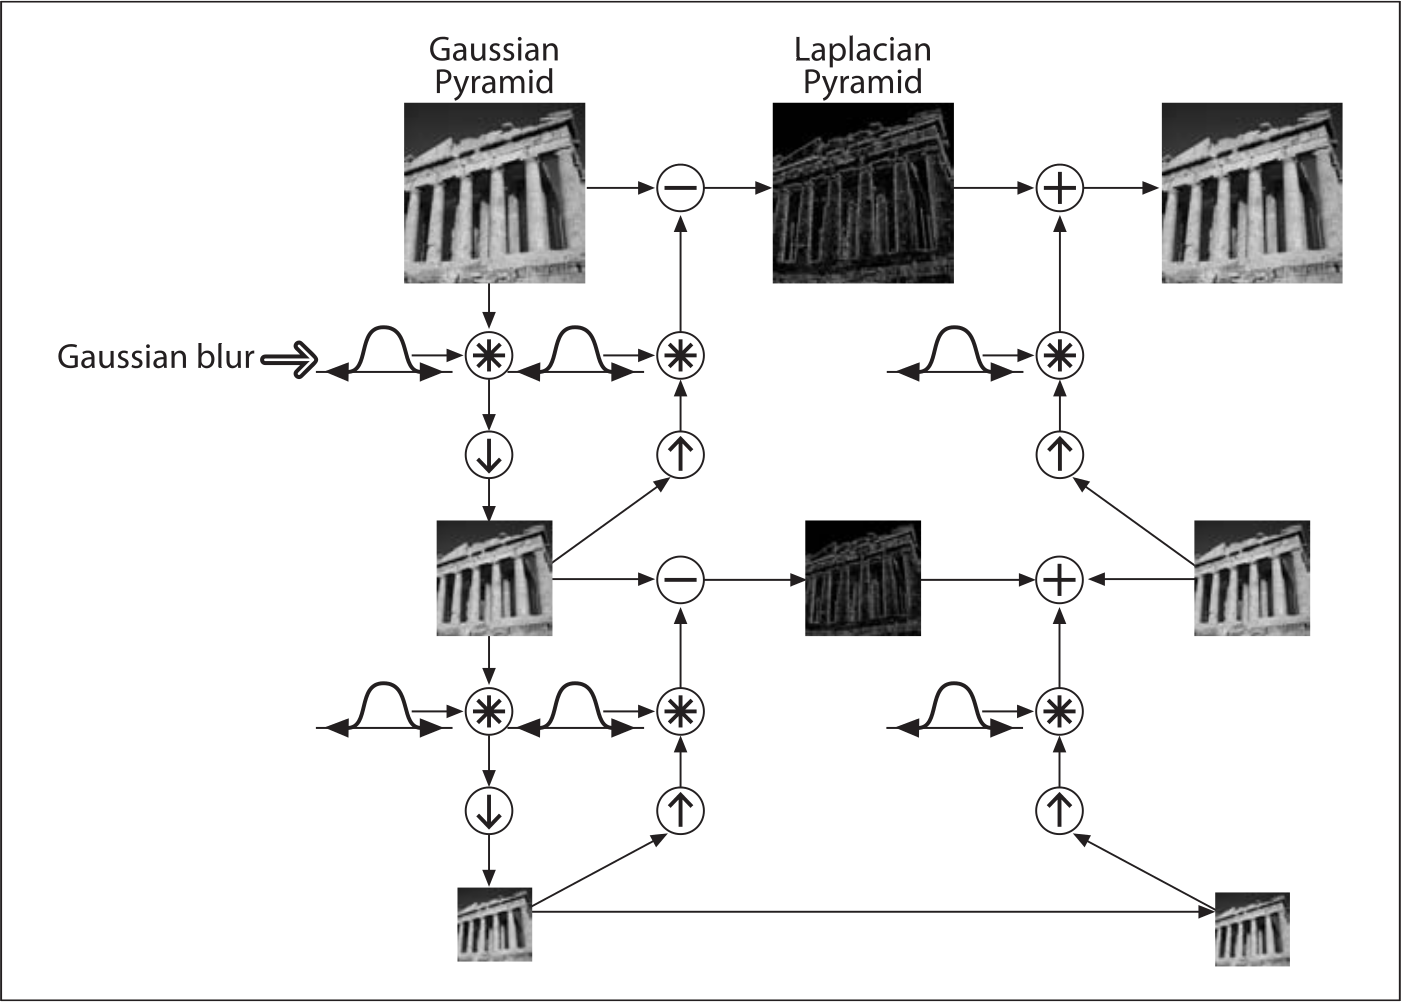
\includegraphics[width=0.8\textwidth]{downsampling.png}
  \caption{Cálculo de las pirámides de Gauss y sus inversas (Laplace). (Bradski y Kaehler)}

  \label{fig:pirámides}
\end{figure}

La figura \ref{fig:pirámides} muestra los pasos involucrados en el cálculo de una pirámide de imágenes y la pirámide laplaciana, que contiene toda la información perdida en cada paso. Si la pirámide de la imagen y la pirámide laplaciana están disponibles, la imagen original puede ser perfectamente reconstruida. En cada nivel de la pirámide, la imagen contiene cuatro veces menos píxeles que la capa inferior (Figura \ref{fig:pirescale}) lo que afectará directamente al tiempo total de procesamiento. 

\begin{figure}
  \centering
  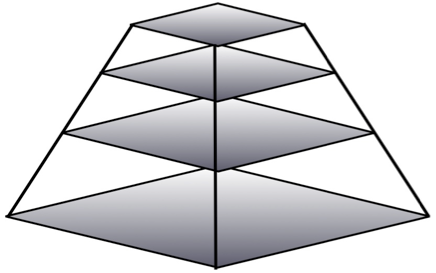
\includegraphics[width=0.5\textwidth]{pyramid.png}
  \caption{Pirámide multiresolución. (journal.code4lib.org)}
  \label{fig:pirescale}
\end{figure}

\section{Detección}
En el contexto de la realidad aumentada, la detección es el proceso de localizar un objeto en una imagen capturada y calcular la posición y orientación de la cámara \emph{(camera pose)} respecto a ese objeto.

Los enfoques que se han dado en las distintas técnicas de detección se pueden clasificar en dos tipos: La detección mediante marcas de referencia o mediante puntos de interés naturales.

\subsection{Detección basada en marcas de referencia \emph{(fiducial markers)}}
Una marca de referencia es un objeto que se coloca en el campo de visión de la imagen a procesar y proporciona un punto de referencia y unas dimensiones conocidas de antemano, facilitando el proceso de detección y el calculo de la pose.

Mediante este método Kato presentó en 1999 un paper que utilizaba marcas cuadradas con un borde negro para calcular la pose de la cámara en tiempo real\cite{Kato}. El resultado fue la biblioteca ARToolKit que ha popularizado la realidad aumentada.

Otros papers en la misma línea, como el de Stricker \cite{Stricker}, en el que describe un método para encontrar las coordenadas 3D de las 4 esquinas de un marcador cuadrado, mientras que Park \cite{Park2} describe un algoritmo para el cálculo de la pose de la cámara a partir de características conocidas.

Hasta el año 2002, las técnicas mediante marcas se habían estudiado ampliamente. Zhang \cite{Zhang} realizo un estudio recopilando y comparando varios de los principales enfoques que existían. A partir de esta fecha no se han presentado nuevos sistemas basados en marcadores.

\subsection{Detección basada en puntos de interés naturales}

El aspecto más importante de la detección de puntos de interés es hacerlo lo más coherente posible. Los mismos puntos de interés que se detectan en un frame, debe detectarse de nuevo en el siguiente cuadro, dado que todavía siguen presentes en la imagen. 

Si tenemos un rectángulo sin bordes en movimiento delante de un fondo del mismo color, sería imposible de rastrear porque el sistema no podría distinguir dos puntos distintos en la imagen. Si tenemos un punto negro sobre un fondo blanco, y esté empieza a moverse, es muy fácil de seguir, ya que el sistema sólo tendría que encontrar ese punto en los siguientes frames. Este punto puede ser visto como una discontinuidad o un punto en el que se produce un cambio busco en la intensidad de la imagen.

Por tanto, el requisito deseable para considerar a un punto de interés es que debe ser una discontinuidad. Si tuviéramos muchos más de estos puntos también sería imposible diferenciar entre ellos y tendríamos el mismo problema que con el rectángulo del mismo color del fondo. Sólo podremos distinguirlos si la región que rodee al punto de interés es diferente, al menos en cierto grado, de la región local que rodea a todos los demás. Por tanto, el segundo requisito de un punto de interés es que él y la región que lo rodea debe ser único. 

Prácticamente en todos los trabajos sobre detección mediante puntos de interés se pueden establecer las siguientes fases:

\begin{description}
\item[Extracción] El proceso de extracción consiste en la búsqueda de zonas en la imagen con diferente apariencia que las que están a su alrededor, denominadas características \emph{(features)}. Normalmente las características suelen ser bordes, esquinas o zonas mas brillantes u oscuras en función del algoritmo utilizado en particular. A esta fase también se la denomina detección.

  Existen muchos algoritmos de detección, que obtienen distintas tipos de características, por ejemplo, el detector de esquinas de Harris\cite{Harris} o el algoritmo FAST \cite{Rosten} que devuelve los píxeles con valores máximos y mínimos en función de sus vecinos mediante técnicas de Machine Learning.

\item[Descripción] Se calcula el vector que describe la característica de un punto significativo para la posterior comparación entre otros puntos de interés. Los enfoques basados en el uso de descripción locales han sido ampliamente investigados y se dividen en dos tipos: el histograma de gradientes y la prueba binaria.

  El histograma de gradientes se calcula a partir de la cuantificación de los gradientes dentro de una área local. En SIFT \cite{Lowe}, una zona se divide en subregiones y se calcula el histograma de gradiente en cada una de ellas. Este enfoque es utilizado y mejorado en los trabajos de Ambai \cite{Ambai}, Bay (SURF) \cite{Bay}, y Wagner \cite{Wagner}

  Una prueba binaria es una comparación de la intensidad de dos píxeles y produce un resultado binario que representa qué píxel es más brillante. Se realizan cientos de pruebas para calcular un vector de características, ya que solo una de ellas no es lo suficientemente discriminatoria. El tema de investigación principal de este enfoque es el de muestreo eficiente entre dos píxeles y es utilizado en los métodos BRIEF \cite{Calonder}, BRISK \cite{Leutenegger}, y ORB \cite{Rublee}. 

\item[Búsqueda de Coincidencias] Los vectores de características se almacenan en una base de datos. Cuando se busca una coincidencia, se accede a la base datos con los datos del vector de consulta y se devuelve el vector almacenado mas similar.

  Si un vector de características es de grandes dimensiones como en SIFT \cite{Lowe}, la búsqueda completa no se podría realizar para tareas en tiempo real. En lugar de ello,  se utilizan técnicas de árboles de búsqueda basado en la aproximación al vecino más cercano \cite{Arya} \cite{Muja}. El costo de la búsqueda de este enfoque depende del número de características almacenados en la base de datos. Otro tipo de búsqueda consiste en mapear el vector de características a un índice de tipo entero \cite{Datar} y almacenarlo en una tabla hash. Este enfoque es teóricamente rápido con $O(1)$, independientemente del tamaño de la base de datos, pero es sensible a errores. Si un vector de características se describe como cadena binaria, se realizará una búsqueda completa en toda la tabla \cite{Calonder}. Para intentar corregir esto, se han planteado la utilización de árboles aleatorios \cite{Lepetit} y estructuras no jerárquicas \cite{Ozuysal}.
\end{description}

Hay muchas clases de detectores de características, pero los más utilizados son los detectores de esquinas (\emph{corners}), de bordes (\emph{edges}) y de regiones (\emph{blobs}). 

\subsubsection{Detector de esquinas de Harris}
El ejemplo más obvio de un punto de interés es una esquina, o la intersección de dos bordes. A lo largo de los años se han desarrollado una serie de algoritmos de detección de esquinas. La mayoría de los algoritmos de detección de puntos de interés calculan una función $C$ de respuesta, ya sea para todos los píxeles, o sólo algunos píxeles seleccionados. 

Probablemente el más famoso detector de esquinas se conoce como ``detector de esquinas de Harris'' desarrollado por Harris \cite{Harris}, que fue creado para la interpretación 3D de secuencias de imágenes. Al igual que con el detector de bordes de Canny, el cálculo de la segunda derivada parcial de una imagen en una dirección específica indicará regiones con cambios bruscos de intensidad de la imagen (discontinuidades) en esa dirección. Dada una imagen en escala de grises en dos dimensiones, $I$, de modo que la intensidad de la imagen en un píxel específico se da por $I(x,y)$, Harris determina $C_{Harris}$ para un punto específico de la siguiente manera: 

En primer lugar, tomamos una región de la imagen encima del área $(u,v)$ y cambiándolo por $(x,y)$. La forma de la región puede ser circular o rectangular. La suma ponderada de las diferencias de los cuadrados (SSD) entre estas dos regiones ,denotada por $S$ y viene dada por:
\begin{equation}
  S(x,y) = \sum_u \sum_v w(u,v) \, \left( I(u+x,v+y) - I(u,v)\right)^2
\end{equation}

$I(u + x, v + y)$ puede aproximarse por una serie de Taylor. Donde $I_x$ y $I_y$ son los gradientes vertical y horizontal de la imagen (derivadas parciales de $I$), tenemos:

\begin{equation}
  I(u+x,v+y) \approx I(u,v) + I_x(u,v)x+I_y(u,v)y
\end{equation}

Esto produce la aproximación:
\begin{equation}
  S(x,y) \approx \sum_u \sum_v w(u,v) \, \left( I_x(u,v)x + I_y(u,v)y \right)^2,
\end{equation}

que se puede escribir en la forma de matriz:
\begin{equation}
  S(x,y) \approx \begin{pmatrix} x & y \end{pmatrix} \textbf{H}_{harris} \begin{pmatrix} x \\ y \end{pmatrix},
\end{equation}

donde  $\textbf{H}_{harris}$ es la \emph{structure tensor},
\begin{equation}
  \textbf{H}_{harris} = \sum_u \sum_v w(u,v) 
  \begin{bmatrix}
    I_x^2 & I_x I_y \\
    I_x I_y & I_y^2 
  \end{bmatrix}
  =
  \begin{bmatrix}
    \langle I_x^2 \rangle & \langle I_x I_y \rangle\\
    \langle I_x I_y \rangle & \langle I_y^2 \rangle
  \end{bmatrix}
\end{equation}

$\textbf{H}_{harris}$ is conocida como la \emph{Matriz de Harris}. Un punto de interés se caracteriza por una variación de $S$ en todas la direcciones del vector $(x,y)$. Si definimos $\lambda_1$ y $\lambda_2$  como los autovalores de la matriz descrita arriba, podemos definir entonces la función de autocorrelación $C_{harris}$  como:

\begin{equation}
  C_{harris} = \lambda_1 \lambda_2 - \kappa \, (\lambda_1 + \lambda_2)^2 = \operatorname{det}(\textbf{H}_{harris}) - \kappa \, \operatorname{trace}^2(\textbf{H}_{harris})
\end{equation}

En función de los autovalores de $\textbf{H}_{harris}$, $\lambda_1$ y $\lambda_2$, podremos distinguir los siguientes casos:
\begin{itemize} 
\item La función tendrá un máximo si ambos autovalores son altos, lo que quiere decir que un desplazamiento en cualquier dirección  va a producir un incremento importante, indicando, por tanto, que se trata de una esquina.

\item La función sera casi nula si ambos autovalores son bajos, es decir que un desplazamiento en cualquier dirección va a producir cambios muy pequeños, por tanto, la región que engloba la subventana es de intensidad constante (pertenece al mismo objeto).

\item Si un autovalor es alto y el otro bajo, entonces, la función tendrá forma de cresta. Por tanto, sólo los desplazamientos en una dirección van a producir pequeños cambios en C(x,y) y cambios significativos en la dirección perpendicular. Esto indicará la presencia de un borde.
\end{itemize}

El valor de $\kappa$ es un parámetro experimental y es determinado empíricamente del rango de 0.04 a 0.15.

\subsubsection{Shi-Tomasi} 
Shi y Tomasi \cite{ShiTomasi} mejoraron el detector de Harris y encontraron que se obtenía un buen resultado en la detección de esquinas, siempre y cuando el autovalor más pequeño era mayor que un cierto umbral. $C_{ShiTomasi} = min(\lambda_{1}, \lambda_{2})$. La función $C_{ShiTomasi}$ tiene el inconveniente de necesitar el cálculo explícito de los autovalores, que costoso computacionalmente. Los autovalores de una matriz de 2x2 se calculan de la siguiente forma: 

\begin{equation}
  \lambda_{12} = \dfrac{1}{2}(trace(\textbf{H}_{harris}) \pm \sqrt{\operatorname{trace}^{2}(\textbf{H}_{harris}) - 4 \operatorname{det}(\textbf{H}_{harris})})
\end{equation}

El cálculo de la raíz cuadrada puede afectar negativamente el tiempo de cálculo. Los resultados muestran que Shi-Tomasi tiene mejor criterio para determinar a un punto de interés, devolviendo más puntos que Harris para un mismo umbral. Los resultados también muestran que Shi-Tomasi es más lento que el algoritmo de Harris para el mismo umbral, posiblemente debido al cálculo de los autovalores. 

\subsubsection{FAST (Features from Accelerated Segment Test)} 
FAST es algoritmo de detección de esquinas presentado por Rosten y Drummond \cite{Rosten}. En contraste con los métodos de detección de puntos de interés, como Harris, FAST tiene un enfoque mucho más cualitativo, y mucho menos costoso, para determinar si un píxel representa una esquina. Para cada píxel, $p$, en una imagen en escala de grises, FAST examina 16 píxeles en un círculo de radio 3 alrededor de $p$, como se muestra en la figura \ref{fig:fast}. La intensidad (valor de gris) de un píxel está dado por $I(x, y)$. FAST simplemente afirma que $p$ puede ser clasificado como un punto de interés si las intensidades de al menos 12 puntos contiguos en el círculo de prueba son más claros o más oscuros que $I(x_p, y_p)$ (la intensidad de p) para un cierto  umbral, $t$. Un punto de interés puede ser categorizado como ``positivo'' (brillante) si por lo menos 12 puntos circulares contiguos tienen intensidades mayores que $I(x_p, y_p) + t$, o ``negativo'' (oscuro) si sus intensidades son más pequeños que $I(x_p , y_p) - t$. Esta partición puede ser útil para que los puntos positivos no sean comparado con puntos negativos en etapas posteriores del tracking.

\begin{figure}
  \centering
  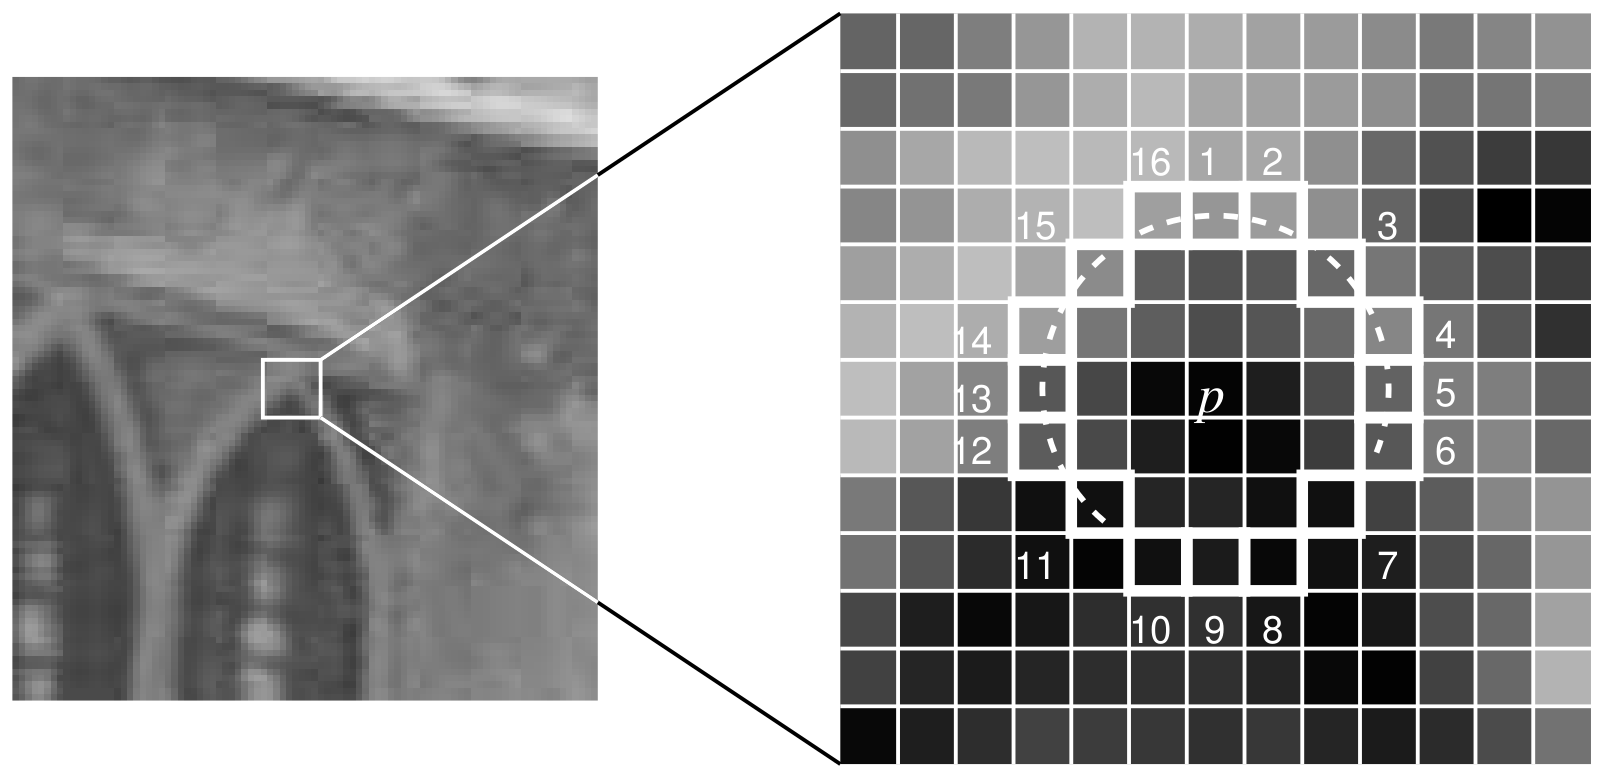
\includegraphics[width=0.8\textwidth]{fast.png}
  \caption{FAST: Círculo de análisis alrededor del píxel $p$. (Rosten y Drummond)
  }
  \label{fig:fast}
\end{figure}

Dado que los 12 puntos deben ser contiguos, la comprobación puede ser acelerada examinando inicialmente soló los píxeles 1, 9, 5 y 13. Un punto de interés sólo puede existir si tres de estos puntos de prueba son todos más brillante o más oscuro que la intensidad de $p$ dado un valor para el umbral. Si más de uno de estos puntos de prueba está  dentro del rango del umbral, $p$ puede ser rechazado de inmediato. Si esta comprobación inicial es satisfactoria, se comprueban el resto de píxeles que quedan en el círculo. Rosten encontró que debido a esta optimización, el algoritmo examina en promedio sólo 3,8 píxeles del círculo para probar si un punto dado es un punto de interés.

De la descripción del algoritmo FAST se puede observar dos potenciales ventajas sobre otros detectores de puntos de interés:
\begin{description}
\item[Rapidez.] Todo lo necesario para procesar una imagen completa es un promedio de 3,8 sumas enteras y comparaciones por píxel. En comparación con otros detectores que requieren el cálculo de derivadas parciales, raíces cuadradas y circunvoluciones, FAST es mucho menos complejo computacionalmente.
\item[Umbralización simple.] El valor del umbral, $t$, es un valor entero que oscila entre 0 y 255 para una imagen en escala de grises de 8 bits. La elección de $t$ influirá directamente en el número, y, posiblemente en la calidad de los puntos de interés detectados. Para aplicaciones en las que es necesario tener un número constante de puntos de interés que deban ser detectados, $t$ puede ser determinado dinámicamente.
\end{description}

Se debe tener en cuenta que estas características conllevan una serie de desventajas en el uso de FAST: 
\begin{enumerate}
\item FAST funciona mal en imágenes borrosas. La mayoría de los detectores de puntos de interés basados esquinas también tienen este inconveniente.
\item FAST no es muy robusto en imágenes que presenten ruido. Se obtiene una alta velocidad de proceso a costa de evaluar una menor cantidad de píxeles por punto, por lo que  no tiene la capacidad para promediar el ruido como en otros detectores que analizan las regiones ponderadas por filtros gaussianos.
\item Pueden ser detectados múltiples puntos de interés juntos. 
\end{enumerate}

El tercer inconvenientes puede ser problema, especialmente si FAST se utiliza para detectar los puntos de interés con los que posteriormente se va realizar un seguimiento (tracking). FAST puede detectar múltiples ``puntos de interés'' alrededor de una esquina en una imagen si está es mayor de uno o dos píxeles. 

En general, es preferible realizar un seguimiento de puntos que se encuentren separados al menos a una cierta distancia entre sí, de modo que las regiones utilizadas para la evaluación no se superpongan. 

FAST prevé este requisito, ofreciendo un paso opcional después de un punto de interés se encuentra el candidato conocido como supresión de no máximos \emph{(non-maximal suppression)}. La supresión de lo no máximos funciona calculando una función de puntuación, $V$ , para cada punto de interés candidato sumando la diferencia de intensidad entre $I(x_p,y_p)$ y cada uno de los píxeles contiguos en el círculo de la prueba que son mas o menos brillante que $I(x_p , y_p)$  dado el  umbral $t$  (aquellos píxeles que pasaron la prueba de 12 puntos). Con la opción de supresión de los no máximos (non-maximal suppression) habilitada, sólo el candidato con la puntuación más alta en una región local es aceptado como un punto de interés. Rosten \cite{Rosten} da la siguiente definición de una función de puntuación $V$:
\begin{equation}
  V = max\left( \displaystyle \sum_{u\in S_{bright}} \left | I(x_u,y_u) - I(x_p,y_p) \right | -t , \sum_{u\in S_{dark}} \left | I(x_p,y_p) - I(x_u,y_u) \right | -t \right) 
\end{equation}

donde $S_{bright}$ y $S_{dark}$ son los conjuntos de píxeles contiguos alrededor de $p$ que son mas brillantes u oscuro que $p$ dado el umbral $t$. Se definen como:
\begin{equation}
  S_{bright} = {{u|I(x_u , y_u ) \geq I(x_p,y_p) + t}}
\end{equation}
\begin{equation}
  S_{dark} = {{u|I(x_u , y_u) \leq I(x_p , y_p ) - t}}
\end{equation}

La eliminación de los no máximos  puede incurrir en una pequeña penalización en el rendimiento en la fase de detección, pero puede conducir a grandes ahorros en los requerimientos computacionales en la función de definición y en la etapa de \emph{matching}.

\subsubsection{Detección de bordes} 
Muchos de los algoritmos de tracking basado en modelos buscan coincidencia entre los bordes de un objeto del mundo real con los bordes de un modelo conocido para determinar la pose. 

Existen gran variedad de algoritmos de detección de bordes, pero uno de los más populares y de mayor éxito es un método perfeccionado por Canny \cite{Canny}. La figura 4.3 se muestra el resultado de la aplicacion del detector de bordes de Canny. Como se puede ver en esta figura, la forma de un modelo se puede estimar mejor si podemos detectar sus los contornos (tanto exteriores como interiores). El detector devuelve un conjunto de curvas conectadas. El tracking de contornos relacionados con la estructura de un objeto de la imagen en lugar realizar un seguimiento de los píxeles individuales reduce significativamente la cantidad de datos a procesar, que es exactamente el propósito de la detección de características. 

El algoritmo de Canny realiza la siguiente secuencia de pasos para realizar la detección de bordes: 
\begin{enumerate}
\item La imagen se difumina ligeramente utilizando un filtro de Gauss (desenfoque) para reducir el ruido que pueden estar presente debido al sensor de imagen (calidad del sensor, aumento de sensibilidad). 
\item Se calcula el gradiente de intensidad de la imagen mediante las primeras derivada parciales respecto a $x$ e $y$. 
\item Un cambio brusco en la intensidad de la imagen podría representar un borde. La busqueda de estas áreas se realiza buscando puntos en los que las derivadas direccionales son máximos locales. 
\item Teniendo en cuenta los puntos anteriores como candidatos para bordes, el área alrededor de cada punto se inspecciona para determinar si en realidad se encuentra en un borde y la dirección del gradiente. Esta etapa se denomina supresión de los no máximos (\emph{non-maximal suppression}) y devuelve el conjunto de puntos del borde. 
\item Los bordes se trazan utilizando umbral de histéresis. La umbralización consiste en imponer un valor umbral, si los píxeles superan ese umbral serán considerados como bordes. Pero aparece un problema si imponemos un umbral muy alto perdemos parte de los bordes, por el contrario si usamos un umbral bajo aparecería ruido, por ello utilizamos la umbralización con histéresis en la que usamos dos umbrales $T_{h}$ y $T_{l}$, siendo $T_{h}$ mayor que $T_{l}$. Después de este paso,se devuelve una imagen binaria donde los píxeles pertenecientes a los bordes están representados por unos y el resto por ceros. 
\end{enumerate}

La imagen binaria devuelta puede procesarse adicionalmente para encontrar curvas y polígonos, pero esto ya no es parte de la etapa de detector de bordes de Canny.

La base de estos métodos es el cálculo de una caracteristica geometrica a partir de los bordes. En el caso del trabajo de Hagbi \cite{Hagbi}, propone un metodo para recononer formas planas y estimar la pose de la cámara a partir del contorno de las formas. Para cada concavidad del contorno, se extraen de las líneas bitangentes, puntos clave invariantes de la proyección. La pose inicial se estima a partir de estos puntos y son refinados mendiante la minimización del error de reproyección.

\subsubsection{Detección de Regiones}
Podemos definir una región \emph{(blob)} como una zona de la imagen que tiene propiedades distintas, como el brillo o el color, comparada con otras zonas que la rodean.   

Dada alguna propiedad de interés expresado como una función de la posición en la imagen digital,

La investigación en este área se centra en algoritmos que podemos agrupar en dos clases principales de detectores de regiones: métodos diferenciales y métodos basados en extremos locales.

Donoser \cite{Donoser} presenta un enfoque para extraer contornos que utiliza MSER (Maximally Stable Extremal Regions) para definir regiones de interes \emph{(blob)}.

\paragraph{MSER - Maximally Stable Extremal Regions}
El detector de regiones extremas MSER (Maximally Stable Extremal Regions) selecciona aquellas regiones cuyos píxeles son más brillantes o más oscuros que todos los píxeles de su alrededor \cite{Matas}. De este modo, las regiones quedan definidas por una propiedad extrema de la función de intensidad en la región y su límite exterior. 
El algoritmo ordena todos los píxeles de la imagen según su intensidad con un coste computacional de $O(n)$ si el rango de los valores de la imagen $S$ es pequeño, por ejemplo los valores de la imagen en escala de grises $\lbrace 0,\ldots,255\rbrace$, ya que la ordenación se implementa mediante un algoritmo BINSORT. Después de la ordenación, los píxeles se colocan en la imagen (con orden ascendente o descendente) y se van creando regiones de componentes conectados que van creciendo y fusionándose (utilizando un algoritmo de tipo \emph{union-find}, con una complejidad temporal de $O(n\,\log(\log n))$) hasta que todos los píxeles han sido seleccionados. Como resultado final se obtienen diferentes funciones de densidad que describen estructuras de datos que representan a cada una de las áreas de los componentes conectados que contiene la imagen.

Las regiones extremas se calculan buscando aquellos componentes conectados que permanecen constantes durante un número determinado de iteraciones. Para ello, se seleccionan como umbrales de las regiones extremas para las diferentes iteraciones los niveles de intensidad que son mínimos locales del rango de cambio de la función del área. Finalmente, el algoritmo transforma en elipses las regiones extremas, que inicialmente pueden tener cualquier forma. 

\subsection{Descriptores de Características}
La búsqueda de correspondencias de punto es una tarea importante para llevar a acabo una triangulación y el cálculo de la pose de la cámara con éxito. Con el fin de encontrar características correspondientes más fotogramas de vídeo que debe ser posible detectar características como se describe en la sección anterior , pero también es importante para identificar las características y relacionarlas entre fotogramas. Llamamos a esta descripción de la función y se trata de extraer información de la característica.

Al igual que con la detección de características , una amplia variedad de algoritmos de descripción de funciones se han presentado en los últimos años . Una buena descripción del carácter debe exhibir estas tres características :

\begin{enumerate}
\item \textbf{Reproducible}  Los descriptores de características deben ser fiables, encontrando los mismos puntos de interés bajo diferentes condiciones de visualización. Debe tener una alta precisión y una tasa baja de falsos positivos. También debe ser invariante a cambios en la rotación, traslación y escala.
\item \textbf{Robusto} El descriptor debe ser capaz de identificar el mismo punto entre los distintos frames, incluso si hay cambios en la iluminación, se presente ruido en la imagen o existan pequeños cambios en el  punto de vista .
\item \textbf{Rápido} Debe ser capaz de extraer información de los puntos característicos y compararla con una gran base de datos en el menor tiempo posible, preferiblemente en tiempo real.
\end{enumerate}

Lowe \cite{Lowe} presenta un método para la extracción de características de la imagen llamado SIFT (Scale Invariant Feature Transform). Este proceso es invariante a cambios en la escala de imagen, traslación y rotación, así también, al menos parcialmente invariante, a cambios en la iluminación y transformaciones proyectivas 3D. Este enfoque transforma una imagen en una gran colección de vectores de características locales llamados  \emph{``SIFT Keys''} que se utilizan para su identificación.

\subsubsection{SURF}
El descriptor SURF, Speeded-Up Robust Features, fue desarrollado por Herbert Bay \cite{Bay} como un detector de puntos de interés y descriptor robustos. El descriptor SURF guarda cierta similitud con la filosofía del descriptor SIFT \cite{Lowe}, si bien presenta notables diferencias que quedarán patentes con la siguiente exposición sobre su desarrollo. Los autores afirman sin embargo que este detector y descriptor presentan principalmente 2 mejoras resumidas en los siguientes conceptos: 
\begin{itemize}
\item Velocidad de cálculo considerablemente superior sin ocasionar perdida del rendimiento.
\item Mayor robustez ante posibles transformaciones de la imagen. 
\end{itemize}
Estas mejoras se consiguen mediante la reducción de la dimensionalidad y complejidad en el cálculo de los vectores de características de los puntos de interés obtenidos, mientras continúan siendo suficientemente característicos e igualmente repetitivos. 

Las diferencias más originales respecto del descriptor SIFT:
\begin{itemize}
\item La normalización o longitud de los vectores de características de los puntos de interés es considerablemente menor, concretamente se trata de vectores con una dimensionalidad de 64, lo que supone una reducción de la mitad de la longitud del descriptor SIFT.
\item El descriptor SURF utiliza siempre la misma imagen, la original. 
\item Utiliza el determinante de la matriz Hessiana para calcular tanto la posición como la escala de los puntos de interés
\end{itemize}

\paragraph{Detección de puntos de interés} 
La primera de las etapas del descriptor SURF es análoga a la del descriptor SIFT en cuanto a la detección de puntos de interés se refiere, si bien el procedimiento para su obtención se basa en diferencias sustanciales que se detallan a continuación. 

El descriptor SURF hace uso de la matriz Hessiana, más concretamente, del valor del determinante de la matriz, para la localización y la escala de los puntos. El motivo para la utilización de la matriz Hessiana es respaldado por su rendimiento en cuanto a la velocidad de cálculo y a la precisión. Lo realmente novedoso del detector incluido en el descriptor SURF respecto de otros detectores es que no utiliza diferentes medidas para el cálculo de la posición y la escala de los puntos de interés individualmente, sino que utiliza el valor del determinante de la matriz Hessiana en ambos casos. Por lo tanto dado un punto $p = (x, y)$ de la imagen $I$ , la matriz Hessiana $H (p, \sigma)$ del punto $p$ perteneciente a la escala $\sigma$ se define como:
\begin{equation}
  H (p, \sigma) = 
  \begin{bmatrix}
    L_{xx} (p, \sigma) & L_{xy} (p, \sigma)  \\ 
    L_{xy} (p, \sigma) & L_{yy} (p, \sigma)
  \end{bmatrix}
\end{equation}
donde $L_{xx} (p, \sigma)$ representa la convolución de la derivada parcial de segundo orden de la Gaussiana con la imagen $I$ en el punto $p$. De manera análoga ocurre con los términos $L_{xy} (p, \sigma), L_{yy} (p, \sigma)$ de la matriz. 

A pesar de que los filtros gaussianos son óptimos para el análisis del espacio-escala, se ha implementado una alternativa a los filtros gaussianos en el detector SURF debido a una serie de limitaciones de estos filtros (como la necesidad de ser discretizados, la falta de prevención total del indeseado efecto aliasing, etc.): los filtros tipo caja (de sus siglas en inglés box-filters). Estos nuevos
filtros aproximan las derivadas parciales de segundo orden de las gaussianas y pueden ser evaluados de manera muy rápida usando imágenes integrales, independientemente del tamaño de éstas. Las imágenes integrales, son calculadas mediante la siguiente fórmula:
\begin{equation}
  I_{\sum}(x,y) = \sum_{i=0}^{i\leq x} \sum_{j=0}^{j\leq y} I(i,j)
\end{equation}
donde $(x, y)$ representan la posición del punto en la imagen y $Ii (x, y)$representa la intensidad de la imagen en el punto. Una vez la imagen integral ha sido creada, se puede calcular la suma de
las intensidades de una región mediante una simple operación:
\begin{equation}
  \sum I = I_{iD} + I_{iA} + I_{iB} + I_{iC}
\end{equation}
De esta forma, el tiempo necesario para el calculo de las operaciones de convolución es independiente del tamaño de la imagen.

El espacio escala del descriptor SIFT descrito anteriormente, se crea a partir de imágenes suavizadas repetidamente mediante la aplicación de un filtro gaussiano y que posteriormente se submuestrean para alcanzar un nivel más alto dentro de la pirámide de dicho espacio escala. Sin embargo en el caso del detector SURF, debido a la utilización de filtros de tipo caja e imágenes integrales, no es necesario aplicar el mismo filtro iterativamente a la salida de una capa filtrada previamente, sino que se pueden aplicar dichos filtros de cualquier tamaño a la misma velocidad directamente sobre la imagen original. De este modo resulta que el espacio escala es analizado mediante la elevación del tamaño del filtro, en vez de reducir el tamaño de la imagen como es el caso del detector SIFT

Las aproximaciones de las derivadas parciales se denotan como $D_{xx} , D_{xy} , y D_{yy}$. En cuanto al determinante de la matriz Hessiana, éste queda definido de la siguiente manera:
\begin{equation}
  det(H_{aprox}) = D_{xx} D_{yy} - (0,9 D_{xy})^2
\end{equation}

donde el valor de 0,9 está relacionado con la aproximación del filtro gaussiano. La imagen de salida obtenida tras la convolución de la imagen original con un filtro de dimensiones 9x9, que corresponde a la derivada parcial de segundo orden de una gaussiana con $\sigma = 1,2$, es considerada como la escala inicial o también como la máxima resolución espacial ($s = 1,2$, correspondiente a una gaussiana con $\sigma = 1,2$). Las capas sucesivas se obtienen mediante la aplicación gradual de filtros de mayores dimensiones, evitando así los efectos de aliasing en la imagen.

El espacio escala para el descriptor SURF, al igual que en el caso del descriptor SIFT, está divido en octavas. Sin embargo, en el descriptor SURF, las octavas están compuestas por un número fijo de imágenes como resultado de la convolución de la misma imagen original con una serie de filtros cada más grandes. El incremento o paso de los filtros dentro de una misma octava es el doble respecto del paso de la octava anterior, al mismo tiempo que el primero de los filtros de cada octava es el segundo de la octava predecesora. De esta manera obtenemos las siguientes series de octavas con sus respectivos filtros.

Finalmente para calcular la localización de todos los puntos de interés en todas las escalas, se procede mediante la eliminación de los puntos que no cumplan la condición de máximo en un vecindario de 3x3x3. De esta manera, el máximo determinante de la matriz Hessiana es interpolado en la escala y posición de la imagen. En este punto se da por concluida la etapa de detección de los puntos de interés.

\paragraph{Asignación de la orientación} 
La siguiente etapa en la creación del descriptor corresponde a la asignación de la orientación de cada uno de los puntos de interés obtenidos en la etapa anterior.
Es en esta etapa donde se otorga al descriptor de cada punto la invarianza ante la rotación mediante la orientación del mismo. 

El primer paso para otorgar la mencionada orientación consiste en el cálculo de la respuesta de Haar en ambas direcciones $x$ e $y$ mediante las funciones representadas en la figura \ref{fig:haar}:

\begin{figure}
  \centering        
  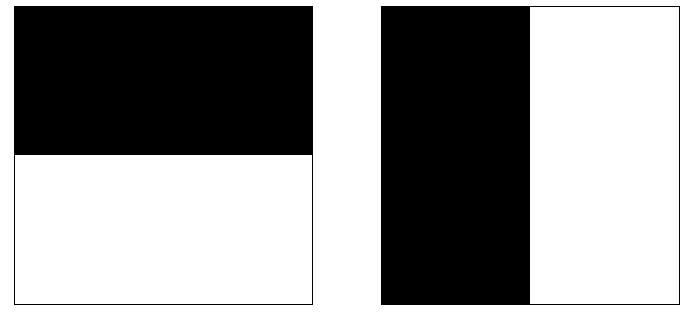
\includegraphics[width=0.5\textwidth]{haar.png}
  \caption{Filtros de Haar empleados en el descriptor SURF. (Bay)}
  \label{fig:haar}
\end{figure}

El área de interés para el cálculo es el área circular centrada en el punto de interés y de radio $6s$, siendo s la escala en la que el punto de interés ha sido detectado. De la misma manera, la etapa de muestreo depende de la escala y se toma como valor $s$. Respecto de las funciones onduladas de Haar, se toma el valor $4s$, por tanto dependiente también de la escala, como referencia, donde a mayor valor de escala mayor es la dimensión de las \emph{wavelets}.

Tras haber realizado todos estos cálculos, se utilizan imágenes integrales nuevamente para proceder al filtrado mediante las máscaras de Haar y obtener así las respuestas en ambas direcciones. Son necesarias únicamente 6 operaciones para obtener la respuesta en la dirección $x$ e $y$. Una vez que las respuestas onduladas han sido calculadas, son ponderadas por una gaussiana de valor $\sigma = 2,5s$ centrada en el punto de interés. Las respuestas son representadas como vectores en el espacio colocando la respuesta horizontal y vertical en el eje de abscisas y ordenadas respectivamente. Finalmente, se obtiene una orientación dominante por cada sector mediante la suma de todas las respuestas dentro de una ventana de orientación móvil cubriendo un ángulo de $\pi/3$ siguiendo las especificaciones recomendadas por el autor. La orientación final del punto de interés será finalmente aquella cuyo vector sea el más grande dentro de los 6 sectores en los que han sido dividida el área circular alrededor del punto de interés. 

\paragraph{Creación del descriptor }
Es en esta última etapa del proceso donde se concreta la creación del descriptor SURF. Se construye como primer paso una región cuadrada de tamaño $20s$ alrededor del punto de interés y orientada en relación a la orientación calculada en la etapa anterior. Esta región es a su vez dividida en 4x4 subregiones dentro de cada una de las cuales se calculan las respuestas de Haar de puntos con una separación de muestreo de 5x5 en ambas direcciones. Por simplicidad, se consideran $d_x$ y $d_y$ las respuestas de Haar en las direcciones horizontal y vertical respectivamente relativas a la orientación del punto de interés. En la Figura \ref{fig:surf2} están representadas tanto las respuestas de Haar en cada una de las subregiones como las componentes $d_x$ y $d_y$ uno de los vectores. Para dotar a las respuestas $d_x$ y $d_y$ de una mayor robustez ante deformaciones geométricas y errores de posición, éstas son ponderadas por una gaussiana de valor $\sigma = 3,3s$ centrada en el punto de interés. En cada una de las sub-regiones se suman las respuestas $d_x$ y $d_y$ obteniendo así un valor de $d_x$ y $d_y$ representativo por cada una de las subregiones. 
Al mismo tiempo se realiza la suma de los valores absolutos de las respuestas $|d_x|$ y $|d_y|$ en cada una de las subregiones, obteniendo de esta manera, información de la polaridad sobre los cambios de intensidad. En resumen, cada una de las subregiones queda representada por un vector $v$ de componentes:

\begin{equation}
  v = (\sum d_x,\sum d_y, \sum |d_x|, \sum |d_y|)
\end{equation}
y por lo tanto, englobando las 4x4 subregiones, resulta un descriptor SURF con una longitud de 64 valores para cada uno de los puntos de interés identificados.

\begin{figure}
  \centering
  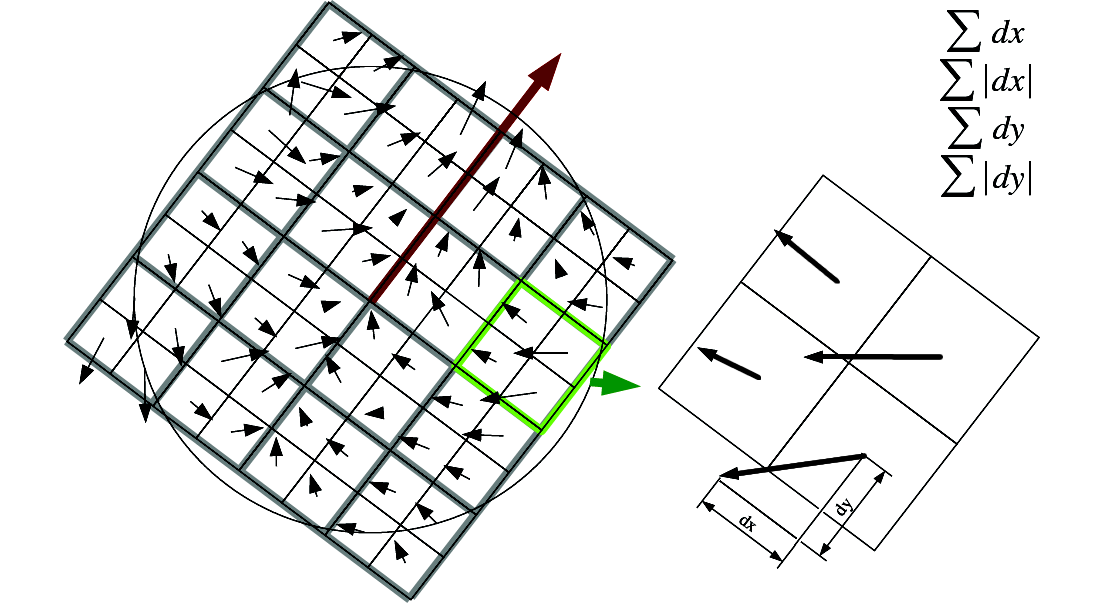
\includegraphics[width=0.5\textwidth]{SURF2.png}
  \caption{Respuestas de Haar en las sub-regiones alrededor del punto de interés. (Bay)}
  \label{fig:surf2}
\end{figure}

\paragraph{Matching entre puntos clave}

Esta sección, al igual que en el caso del descriptor SIFT, representa la correspondencia de los puntos clave identificados entre dos imágenes. La estrategia utilizada para establecer las correspondencias entre los puntos clave de ambas imágenes es la de ``el vecino más próximo'' descrita anteriormente. En el caso del descriptor SURF, el umbral relativo es fijado con un valor de 0,7.

\begin{figure}
  \centering        
  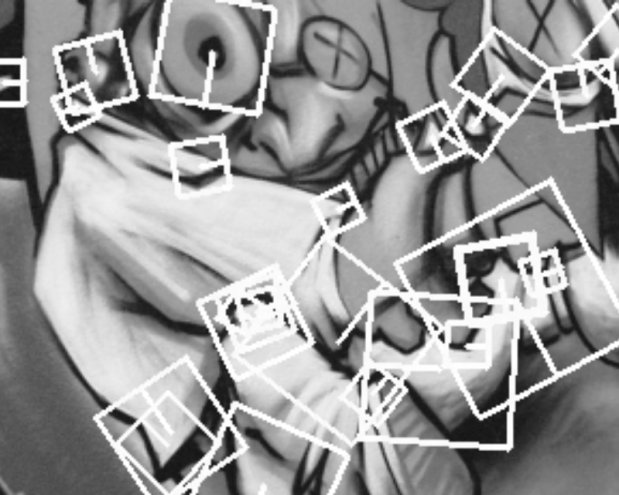
\includegraphics[width=0.5\textwidth]{SURF1.png}
  \caption{Estimación de la orientación sobre puntos de interés. (Bay)}
  \label{fig:SURF1}
\end{figure}

\section{Tracking}
En contraste con la detección, que estima la pose de la cámara en una imagen, el tracking es el seguimiento del objeto (y la estimación de la pose de la cámara respecto a ese objeto) en una secuencia de fotogramas.

El procedimiento a seguir es la de identificar ``puntos clave'' visualmente significativos en un frame que podamos encontrar de forma fiable de nuevo en el siguiente. El procedimiento de tracking se basa en encontrar una cantidad suficiente de estas correspondencias de puntos entre los frames.

El tracking, es un problema complejo debido a la pérdida de información causada por la proyección del mundo 3D en una imagen 2D, la calidad de la imágenes obtenidas, fondos difíciles de segmentar, oclusiones totales o parciales, cambios en la iluminación y la exigencia de para trabajar en tiempo real. 

Para construir un buen sistema de tracking, es deseable que cumpla con los siguientes requisitos:

\begin{description}
\item [Robusto] Incluso en condiciones complicadas, como fondos difíciles de segmentar, cambios de iluminación, oclusiones o movimientos complejos, un algoritmo de tracking debe ser capaz de seguir al objeto de interés.

\item [Adaptable] Adicionalmente a los cambios de entornos que se puedan producir, el objeto en sí también puede sufrir cambios. Esto requiere que el algoritmo tenga algún mecanismo de adaptación para el seguimiento del objeto según la apariencia que tenga en cada momento.

\item [Cómputo en tiempo real] Para obtener una sensación fluida y que el ojo humano no perciba retrasos en la imagen, al menos debemos trabajar y procesar 15 imágenes por segundo. Por tanto, es necesario que el algoritmo sea rápido y esté optimizado.

\end{description}

Desde el punto de la información obtenida para el cálculo de la pose de la cámara, las técnicas de tracking se pueden se dividir en dos tipos:

\begin{description}
\item [Tracking por detección o búsqueda (by matching).] El cálculo de la posición y orientación de la cámara (camera pose) se realiza en cada frame por correspondencia entre la imagen de entrada y otra de referencia mediante una técnica de detección. La información de anteriores “poses” de la cámara no son tenidas en cuenta para la estimación de la nueva pose. El calculo de la pose mediante arboles aleatorios \cite{Lepetit} y estructuras no jerárquicas \cite{Ozuysal} son ejemplos de este tipo de enfoque.

\item [Tracking mediante tracking.] Para el calculo, la pose previa es utilizada como pose inicial para el cálculo de la posición y orientación actual. Una vez que se detectado un objeto, se hace un seguimiento de los puntos claves del objetos en el siguiente fotograma \cite{Wagner}, o minimizan la diferencia entre dos imágenes consecutivas \cite{Park} y analizan el cambio no lineal de iluminación producida \cite{Dame}. La mayoría de estos enfoques se basan en la minimización del desplazamiento de la cámara entre dos imágenes sucesivas.

\end{description}

Otra clasificación de los métodos de tracking disponibles puede dividirse en dos clases: basado en detección de características y basados en detección de modelos.

\subsection{Tracking por detección de características \emph{(feature-based)}}
En el mundo de la visión artificial una característica (feature) es una zona de la imagen que un algoritmo de tracking puede detectar y seguir a lo largo de múltiples frames. Normalmente las características suelen ser bordes, esquinas, zonas mas brillantes u oscuras en función del algoritmo de tracking en particular.

En lugar de utilizar marcadores de referencia, la estimación de la pose de la cámara se puede realizar mediante la extracción de características naturales, como puntos, líneas, bordes o texturas. Esta línea de investigación también ha sido ampliamente estudiado. Park \cite{Park3} presenta un método en el que utiliza las características naturales como una extensión en el tracking de características artificiales. Después de realizar el cálculo de la estimación de la pose de la cámara mediante características visuales conocidos, el sistema sistema adquiere dinámicamente características naturales adicionales y los utiliza para la actualización continua de la estimación de la nueva pose. De esta manera proporciona un seguimiento robusto, incluso cuando las marcas originales originales ya no están a la vista.

\subsubsection{Optical Flow}
El \emph{Optical Flow} o flujo óptico juega un papel importante en la estimación y descripción del movimiento, por lo cual es comúnmente utilizado en tareas de detección, segmentación y seguimiento de objetos móviles en una escena a partir de un conjunto de imágenes. 

El flujo óptico puede ser definido como el movimiento aparente de los patrones de intensidad en una imagen. La palabra aparente indica que el movimiento espacial de los objetos (campo de movimiento) puede coincidir o no con el flujo estimado. No obstante, en situaciones en las cuales el movimiento de los objetos implica un movimiento de sus patrones de intensidad en el plano imagen, el flujo óptico puede ser directamente relacionado con el movimiento de los objetos en la escena. La mayoría de las técnicas existentes para la estimación del flujo óptico se puede clasificar en 4 categorías: las basadas en gradientes espacio-temporales, las basadas en comparación de regiones, las basadas en fase y las basadas en energía.

En todas las estrategias de estimación de flujo óptico se parte de la hipótesis de que los niveles de gris permanecen constantes ante movimientos espaciales en un tiempo dado. Dicha hipótesis da lugar a la ecuación general de flujo óptico, donde $I(x, y, t)$ corresponde a la intensidad en niveles de gris del píxel $(x,y)$ de la imagen $I$ en el tiempo $t$. 
\begin{equation}
  I(x,y,t) = I(x+dx,y+dy,t+dt)
\end{equation}

Expandiendo la ecuación anterior en series de Taylor sobre el punto $(x,y,t)$
\begin{equation}
  I(x,y,t) = I(x,y,t) + dx \frac{\partial I}{\partial x}+dy\frac{\partial I}{\partial y} + dt \frac{\partial I}{\partial t} + \epsilon
\end{equation}

donde $\epsilon$ contiene la información de las derivadas de orden superior. Si se asume $\epsilon$ despreciable, la ecuación de flujo óptico puede reescribirse como
\begin{equation}
  I_xu +I_yv+I_t = 0
\end{equation}
donde $(u,v)$, con $u = dx/dt$ y $v = dy/dt$ , corresponde al vector de flujo óptico y, $I_x$ y $I_y$ son las derivadas parciales horizontal y vertical de la imagen, respectivamente. Para cada píxel $(x,y)$ de la imagen, en el tiempo $t$, puede plantearse la ecuación anterior, sin embargo no existe una única solución para esta ecuación. Diferentes restricciones pueden emplearse para estimar el flujo óptico en la imagen. Horn y Shunck en \cite{Horn} restringen el flujo óptico en la imagen a variar suavemente, por lo que la ecuación es minimizada junto a un término de regularización que penaliza los cambios abruptos del flujo. Lucas y Kanade (LK) \cite{LKanade} proponen un método alternativo que se describe a continuación el cual puede ser implementado de forma más eficiente que el propuesto en \cite{Horn}. Las técnicas propuestas en \cite{Horn} y \cite{LKanade} se basan en gradientes espacio-temporales pues minimizan la ecuación anterior. 
\begin{figure}
  \centering
  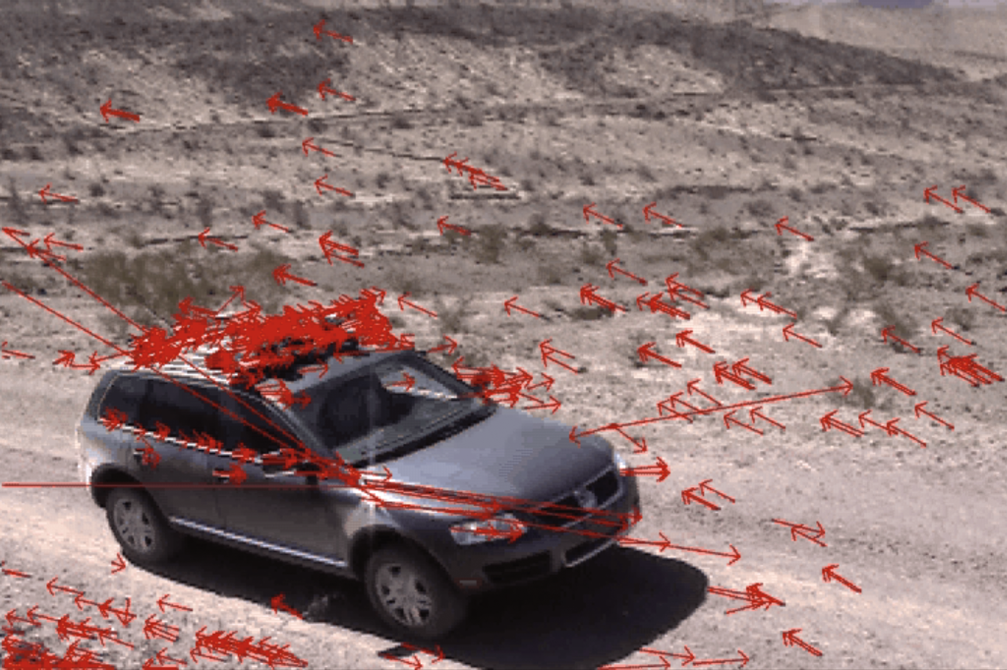
\includegraphics[width=0.8\textwidth]{LK.png}
  \caption{Lucas-Kanade: Seguimiento de puntos. (David Stavens)}
  \label{fig:overviewLK}
\end{figure}

\paragraph{Lucas-Kanade}
Este método asume que el flujo óptico es constante sobre una región. Sea $R$ una región de la imagen y $(u,v)$ su vector de flujo óptico asociado, entonces se cumple para cada píxel de la región, es decir
\begin{equation}
  I_x(p_i)u+I_y(p_i)v = -I_t(p_i) \quad  \forall p_i \in R
\end{equation}
Organizando el conjunto de ecuaciones en forma matricial
\begin{equation}
  A=
  \begin{bmatrix}
    I_x(p_1) & I_y(p_1) \\
    I_x(p_2) & I_y(p_2) \\
    \vdots  & \vdots  \\
    I_x(p_n) & I_y(p_n) 
  \end{bmatrix}
  \quad
  d=
  \begin{bmatrix}
    u\\
    v
  \end{bmatrix}
  \quad
  b = -
  \begin{bmatrix}
    I_t(p_i) \\
    I_t(p_2) \\
    \vdots  \\
    I_t(p_n)
  \end{bmatrix} 
\end{equation}

donde la matriz $A$ contiene las derivadas espaciales de la imagen, el vector $d$ corresponde al vector de flujo óptico $(u,v)$ y el vector $b$ contiene las derivadas temporales de la imagen.

Pre-multiplicando (3) por la transpuesta de $A$ se tiene
\begin{equation}
  A^T A d =A^T b
\end{equation}
donde el vector de flujo óptico es encontrado como 
\begin{equation}
  d= (A^T A)^{-1} A^T b
\end{equation}
El cálculo del flujo óptico implica la inversión de la matriz 
\begin{equation}
  A^TA=
  \begin{bmatrix}
    \sum I_x I_x  & \sum I_x I_y \\
    \sum I_y I_x  & \sum I_y I_y      
  \end{bmatrix}
\end{equation}

por la cual la solución existe si la matriz $A^TA$ es invertible y bien condicionada. Shi y Tomassi definen en [13] las propiedades que debe cumplir una región para que el flujo óptico se estimado apropiadamente utilizando la técnica de LK. Sean $\lambda_1$ y $\lambda_2$ los valores propios de la matriz  $A^TA$ para cierta región $R$ de la imagen, entonces se debe cumplir que:
\begin{itemize}
\item $min(\lambda_1 , \lambda_2) > \lambda_{min} \in R^+$ , lo cual garantiza que $A^TA$ es invertible y la región no es ruidosa.
\item $\lambda_1 /\lambda_2 < \tau$, lo que garantiza que $A^TA$ está bien condicionada y no se presenta bordes en una sola dirección
\end{itemize}

Bajo estas 2 condiciones el flujo óptico puede ser apropiadamente estimado. En la práctica existen ciertos factores que pueden inducir errores en la estimación. Entre ellos se encuentran la variación temporal de los niveles de gris sobre la región, desplazamientos grandes de la región entre las imágenes consecutivas e incoherencia de movimiento. El primero es independiente de la técnica de LK pero los otros 2 factores pueden ser controlados seleccionando un tamaño apropiado para la región R. Una región pequeña en comparación al tamaño del objeto garantiza una consistencia en el movimiento de las intensidades de gris, sin embargo si el objeto se desplaza rápidamente, éste puede salir de la región lo que produce un error en la estimación del flujo óptico. Por tal motivo existe un compromiso en el tamaño de la región R, el cual puede ser manejado con una implementación piramidal que estime  secuencialmente el flujo en diferentes escalas. En \cite{Bouguet} se presenta una implementación piramidal de la técnica de LK en la cual el flujo óptico es calculado recursivamente sobre versiones de diferentes escalas de las imágenes. En principio el flujo es estimado sobre imágenes en una escala baja para permitir grandes desplazamientos, posteriormente la escala se reduce para realizar una estimación más precisa  y evitar inconsistencias de movimiento. El tamaño de la región se mantiene fijo sobre todas las escalas.

\subsection{Tracking por detección modelos \emph{(model-based tracking)}}
La tendencia más reciente en las técnicas de tracking es el basados en modelos. Estas técnicas utilizan explícitamente un modelo de las características de los objetos rastreados, como por ejemplo, un modelo CAD 2D o un patrón del objeto basado en sus características distinguibles. El primer trabajo basado en modelos fue obra de Comport \cite{Comport} que en 2003 que utilizó una aproximación visual porción adaptada de la robótica para el cálculo de la cámara pose de una gama de características de modelo ( líneas, círculos , cilindros y esferas). 

\section{Reconocimiento y análisis de documentos}

\subsection{Texto y documentos}
En general, podemos considerar que cualquier escena o imagen que tenga un contenido textual como si fuera un documento. Esto incluiría tanto un libro, la matricula de un vehículo o un cartel en una pared. La mayoría de trabajos mediante cámaras están basados en la extracción de texto en imágenes fijas o secuencias de vídeo en las que los autores denominan imágenes naturales, en lugar de imágenes donde el texto está estructurado como los documentos. Ambos enfoques tienen sus desafíos y distintos modos de acometerlos, pero el objetivo final de todos es la de dotar a las cámaras la capacidad de lectura.

En el caso de documentos estructurados, que es el del dominio de este trabajo, las imágenes suelen ser documentos impresos como artículos, cartas, formularios o páginas de libros, donde gran parte de la imagen se asume que es texto, pero también puede contener figuras, diagramas e incluso algunos autores han tratado con anotaciones escritas a mano \cite{Chen}

\subsection{Identificación y recuperación de documentos}
Aunque hoy en día la mayor parte de la producción de información en forma de documentos se realiza por medio de herramientas informáticas (procesadores de texto, correo electrónico, etc.), puede ocurrir, y de hecho será un caso muy habitual, que la información no se restrinja a documentos actuales, ya automatizados, sino que se encuentre impresa. Incluso puede ocurrir que nos interese disponer sólo de la información antigua (archivos y manuscritos).

En estos casos para conseguir una gestión eficaz y ágil, es necesario digitalizar previamente estos documentos para incorporarlos al sistema que tenga implementado la organización.

Las primeras aplicaciones se basaban en el paradigma de reconocimiento de caracteres (OCR), donde se utilizaban estas técnicas para realizar un análisis del contenido informativo de los documentos y utilizarlo para su clasificación y almacenamiento. 

La recuperación de objetos (también nombrada por otros autores reconocimiento o identificación) se incorpora recientemente en la detección de tal manera que un objeto es capturado en una imagen, recuperado de una base de datos y su pose inicial se calcula simultáneamente \cite{Pilet}

El desarrollo de la investigación realizada en este ámbito se inició con los métodos que utilizaban marcas especiales en el documento, como códigos de barras \cite{Graham} o glifos para vincular contenido electrónico con las imágenes capturadas \cite{Hecht}. Los inconvenientes de estos enfoques es que es necesario modificar el formato y la apariencia del documento para introducir las marcas, que en algunos casos pueden distraer al usuario del contenido del documento. Por otro lado, un documento válido para el sistema al que no se le hayan incluido previamente estas marcas, no será detectado y vinculado con la información a recuperar.

La utilización del teléfono móvil y otros dispositivos portátiles para la identificación de documentos ha hecho que publiquen diversos artículos con algoritmos y métodos que parten de las propias limitaciones de estos dispositivos como es la baja capacidad de computo, la calidad de las imágenes capturadas, en muchos casos borrosas, y la captura parcial del documento.

Las técnicas de identificación y recuperación de documentos se pueden dividir en dos categorías \cite{Peng}: basados en la búsqueda de coincidencias de características locales y las que, además de lo anterior, utilizan la distribución del contenido dentro de la página.

\subsubsection{Basados en la búsqueda de coincidencias de características locales (feature matching)}
Algunos autores proponen técnicas de detección basados en la extracción de características invariante similares a SIFT \cite{Lowe} o SURF \cite{Bay} en trabajos como \cite{Yang} \cite{Psyllos} \cite{Brown} aplicadas a imágenes naturales y en alta resolución. Sin embargo, como indican Uchiyama y Saito \cite{Uchiyama}, estos métodos no funcionan correctamente para la identificación de documentos, ya que no presentan zonas de textura y se producen patrones binarios repetitivos (el texto de un documento cumple esta disposición). 

Mediante una variación del proceso inspirado en la metodología de Lowe \cite{Lowe} y Bay \cite{Bay}, Augereau \cite{Augereau} obtiene buenos resultados sobre documentos semi-estructurados (billetes de tren, tickets,...) realizando una selección de los puntos extraídos y una adaptación del algoritmo RANSAC para la validación de supuestos aciertos en la comparación.

\begin{figure}
  \centering
  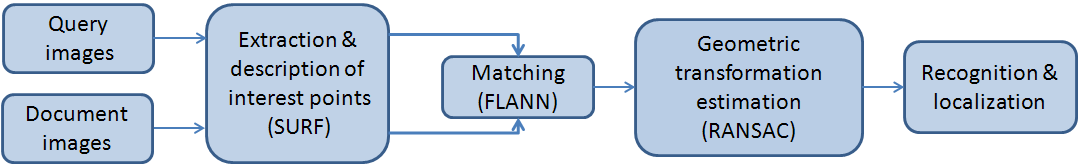
\includegraphics[width=0.9\textwidth]{standardObject.png}
  \caption{Proceso habitual para reconocimiento de imágenes mediante descriptores SURF (Augereau)}
  \label{fig:extraccionSt}
\end{figure}

\begin{figure}
  \centering
  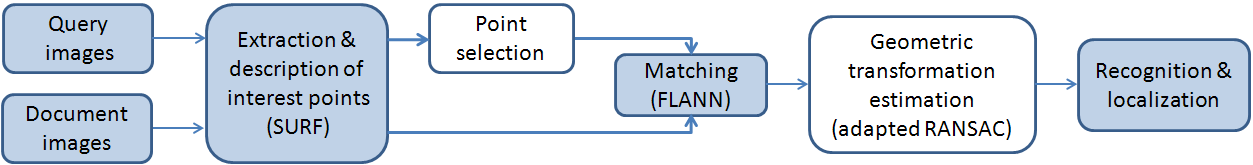
\includegraphics[width=0.9\textwidth]{adaptedObject.png}
  \caption{Proceso adaptado para reconocimiento de documentos mediante SURF (Augereau)}
  \label{fig:extraccionAd}
\end{figure}

El algoritmo tiene una alta tasa de recuperación y precisión, es robusto a las deformaciones que pueda tener la imagen (perspectiva) y no necesita ningún paso previo de segmentación, pero no funciona ante grandes secciones de texto y la identificación es para obtener documentos similares (no idénticos) a la imagen utilizada como consulta.

En PaperUI, Liu y Liao \cite{LiuLiao} implementan hasta siete enfoques distintos para identificar un documento: códigos de barras, micro-patrones ópticos, codificación oculta, huella digital, reconocimiento óptico de caracteres, detector de características locales como SIFT y FIT (una variación de SIFT), incluso tecnología RFID. Sin embargo PaperUI no es capaz de manejar bases de datos de gran tamaño porque el almacenaje de los vectores de características de SIFT requiere gran cantidad de memoria. 


\subsubsection{Basados en combinación coincidencias de características locales y la distribución del contenido dentro de la página}
Para superar las limitaciones, que tienen los enfoques anteriores en el uso específico de imágenes de documentos, otros autores proponen metodologías diseñadas para la recuperación de documentos, haciendo uso explícito de las características inherentes de la estructura del documento y el texto que contiene.

En su articulo, Liu y Doermann \cite{Liu}, presentan un método de recuperación basado en pares y tríos de tokens. En este método, se captura una página mediante un teléfono móvil y se envía a un servidor para recuperar el documento correspondiente. La aplicación ha sido desarrollada para trabajar con bases de datos de gran tamaño, sin embargo, se necesita mucho tiempo de procesamiento, alrededor de 4 segundos por consulta. Este tiempo de respuesta  supone un punto bastante negativo para considerarlo introducir en aplicaciones en tiempo real.

\emph{HotPaper} de Erol \cite{Erol}, es otro método que utiliza las características locales extraídas del texto del documento y su distribución denominado \emph{Brick Wall Coding Features (BWC)}. BWC define una característica local mediante la delimitación de palabras. Esta codificación es invariante a cambios de escala y robusta ante ligeras distorsiones de la perspectiva. El tiempo de procesamiento es rápido, alrededor de 300 ms por consulta y puede reconocer documentos a partir de imágenes con tan solo 4-5 líneas de texto y tamaños de imagen de 176 x 144. Como inconvenientes presenta problemas de escalabilidad, ya que el tamaño de la base de datos es muy pequeña, menos de 5000 páginas y la tasa de precisión es sólo alrededor del 60\%. 

Utilizando el mismo enfoque, pero utilizando otra codificación para generar los descriptores a partir de los \emph{bounding boxes}, Moraleda \cite{Moraleda} mejora la precisión hasta casi el 90\% y la escalabilidad para poder trabajar hasta con 500.000 documentos almacenados. 

\begin{figure}
  \centering
  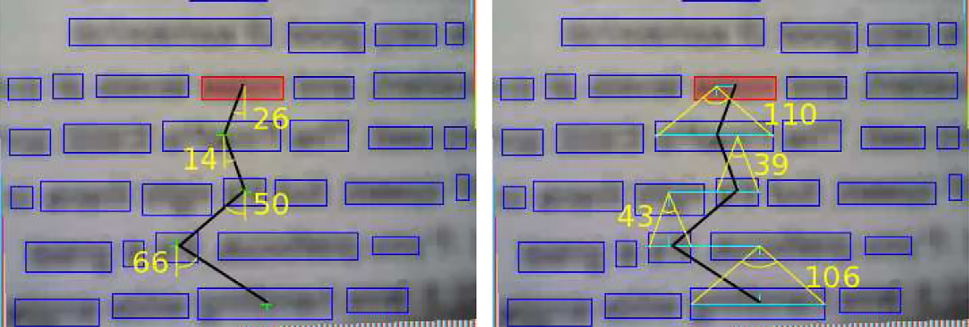
\includegraphics[width=0.9\textwidth]{bwcBounding.png}
  \caption{BWC: \emph{Bounding Boxes} en un fragmento de texto  (Moraleda)}
  \label{fig:extraccionAd2}
\end{figure}

Nakai y Kise proponen un método llamado \emph{Locally Likely Arrangement Hashing (LLAH)}, que utiliza el centro de una palabra como un punto característico y calcula descriptores locales basados en estos puntos\cite{Nakai}. LLAH tiene una alta escalabilidad y el esquema de indexación y recuperación empleado es extremadamente rápido. Los autores han confirmado que LLAH tiene una tasa de acierto del 99\% y con un tiempo de procesamiento de 50 ms en una base de datos de 20 millones de páginas.

En el algoritmo LLAH original, el movimiento de la cámara está restringido, ya que los cambios en el punto de vista causan variaciones en los descriptores locales. Uchiyama \cite{Uchiyama2} salva esta limitación estudiando el comportamiento de los descriptores al variar el punto de vista y actualizándolos continuamente. Como resultado, el método puede aplicarse a varias posiciones e inclinaciones de la cámara, permitiendo un movimiento de la cámara mucho más flexible. Iwata \cite{Iwata} extiende también el algoritmo LLAH para su utilización con imágenes parciales del documento en las que aparezcan tan sólo 4 o 5 líneas de texto. Por otra parte, a través del proceso de recuperación, LLAH puede estimar la \emph{pose} de la imagen de búsqueda en el documento electrónico, que es muy útil para mostrar información relevante sobre el documento.

Esta técnica también ha sido aplica para el desarrollo de marcadores de puntos aleatorios \cite{Saito}

\subsection{Locally Likely Arrangement Hashing (LLAH)}

LLAH es un método ampliamente utilizado para la recuperación de imágenes de documentos. El algoritmo se ha tomado como base para otras aproximaciones, revisado y mejorado, tanto por sus autores, como por otros investigadores. En este apartado estudiaremos el algoritmo original que presentaron los autores \cite{Nakai0}

\begin{figure}
  \centering
  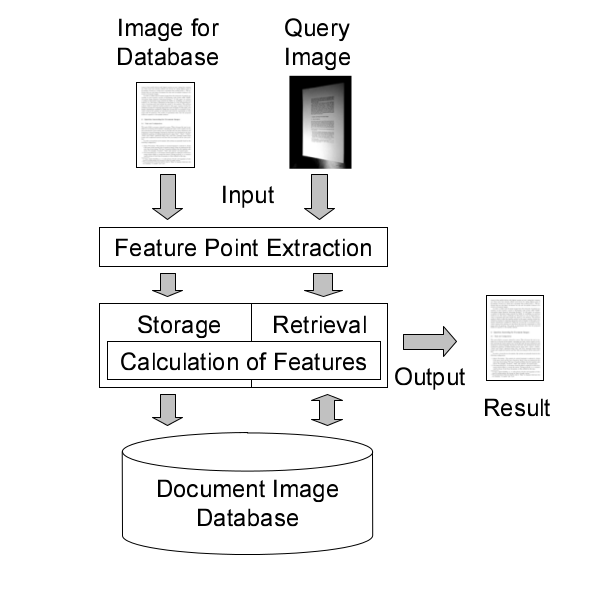
\includegraphics[width=0.6\textwidth]{LLAHesquema.png}
  \caption{LLAH: Visión General del proceso (Nakai y Kise)}
  \label{fig:overview}
\end{figure}

La Figura \ref{fig:overview} muestra un esquema general del proceso. En la etapa de extracción, la imagen se transforma en un conjunto de puntos de características. A continuación, los puntos se pasan a la etapa de almacenamiento o de recuperación (en función de la tarea  realizar). Estos pasos comparten la etapa de cálculo de características. En la etapa de almacenamiento, cada punto se almacena de forma independiente en la base de datos de imágenes de documentos usando su característica. La imagen es indexada utilizando cada uno de los puntos de características. En el paso de recuperación, se accede al  documento mediante las búsqueda de los puntos encontrados.

\subsubsection{Extracción de puntos característicos}
Un requisito importante en la extracción de características es que los puntos se deben obtener de forma idéntica, bajo la misma distorsión de perspectiva, ruido y resolución. Para satisfacer este requisito, emplean como puntos característicos los centroides de las regiones que ocupan las palabras del documento.

En primer lugar, se realiza una umbralización adaptativa a la imagen de entrada (Fig.\ref{fig:extraccion}(a)) y así obtener una imagen binaria (Fig.\ref{fig:extraccion}(b)). A continuación, se desenfoca usando un filtro gaussiano. Seguidamente, la imagen desenfocada es umbralizada de nuevo (Fig.\ref{fig:extraccion}(c)). Las regiones resultantes se supone que son espacios ocupados por palabras, y por último, (Fig.\ref{fig:extraccion}(d)) se extraen los centroides de las regiones para utilizarlos como puntos característicos.

\begin{figure}
  \centering
  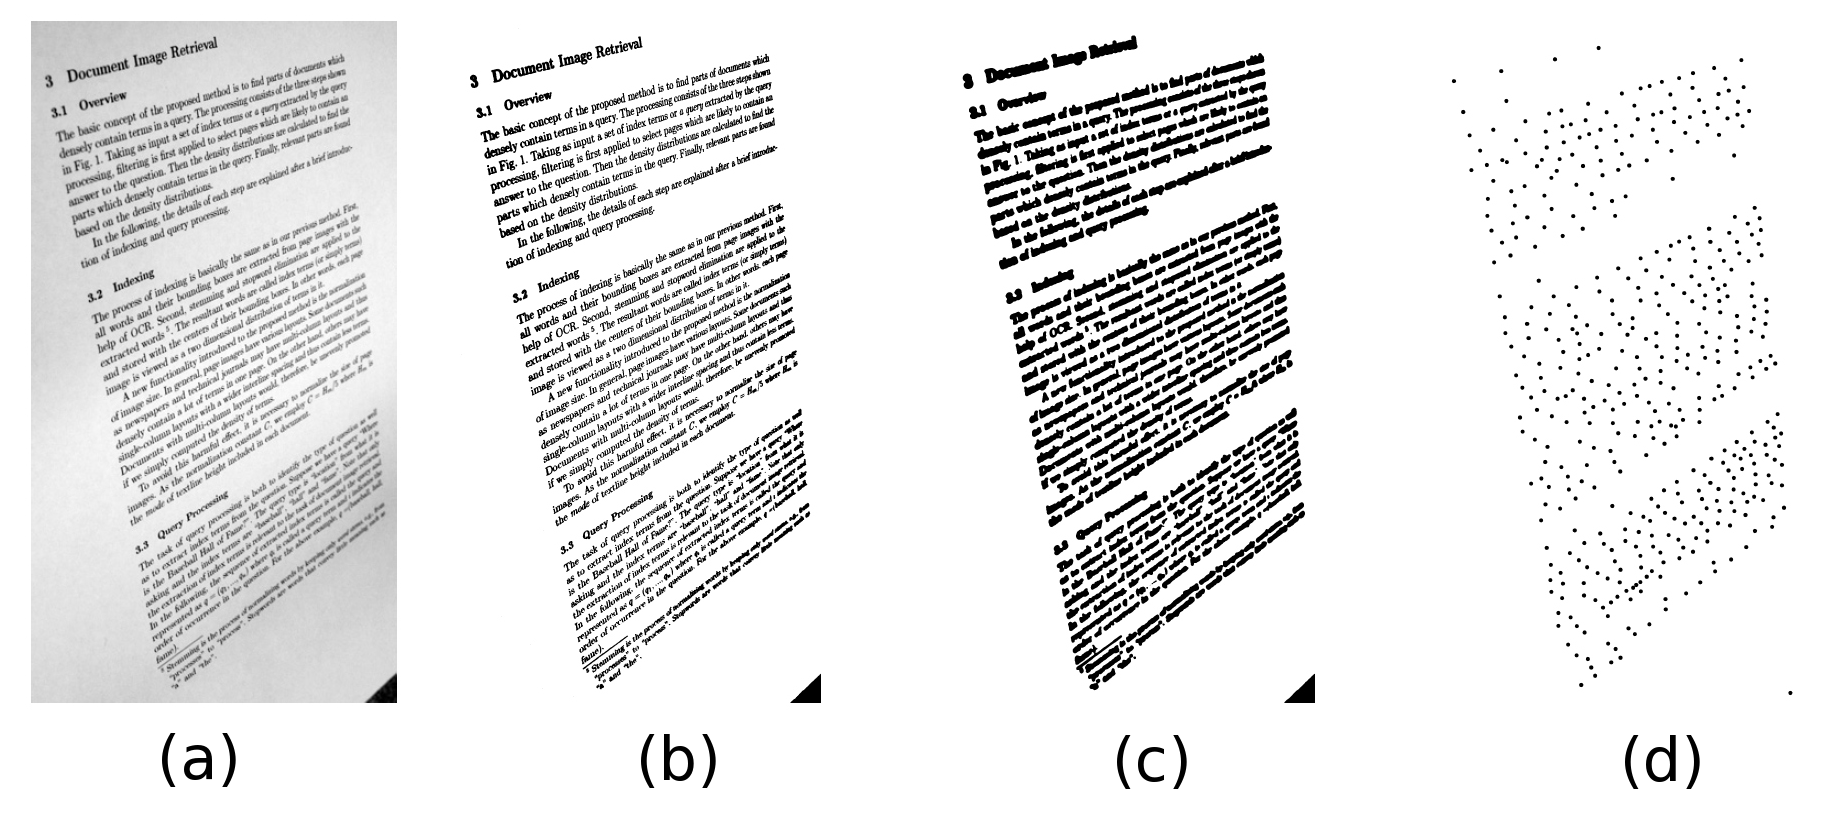
\includegraphics[width=0.9\textwidth]{LLAH.png}
  \caption{LLAH: Extracción de características (Nakai y Kise)}
  \label{fig:extraccion}
\end{figure}

\subsubsection{Cálculo de Descriptores locales}
Los descriptores de LLAH tiene las siguientes características:
\begin{itemize}
\item Se define un descriptor para cada punto característico. Con el fin de obtener robustez y disponibilidad en situaciones de oclusión, un descriptor tiene una localización.
\item Se calcula utilizando invariantes geométricos. Una invariante afín se define mediante cuatro puntos coplanares ABCD de la siguiente manera:
  \begin{center}
    $ \dfrac{P(A,C,D)}{P(A,B,C)} $
  \end{center}
  donde P(A,B,C) es el área de un triángulo con vértices A, B y C.
\item Un descriptor consta de más de una invariante geométrico. Para aumentar el poder de discriminación de un descriptor, se utilizan múltiples invariantes afines calculados a partir de varios puntos característicos. Cómo un invariante afín se calcula a partir de cuatro puntos, podemos calcular más de una invariante partir de más de cuatro puntos característicos. En concreto, un descriptor es $(r_{(0)},...,r_{_{m}C_{4}-1})$ calculado a partir de los $m$ puntos contiguos donde $r_{(i)}$ es una invariante afín. Se utilizan todas las posibles combinaciones de cuatro puntos $m$.
\item Se calculan más de un descriptor para cada punto característico. Con el fin de hacer frente a los errores de la extracción de puntos característicos,se calculan múltiples descriptores a partir $n (>m)$ puntos mas cercanos. En concreto, se calculan $_{n}C_{m}$ descriptores, todas las combinaciones posibles de $m$ puntos contiguos sobre $n$ puntos totales.
\end{itemize} 

\begin{figure}
  \centering
  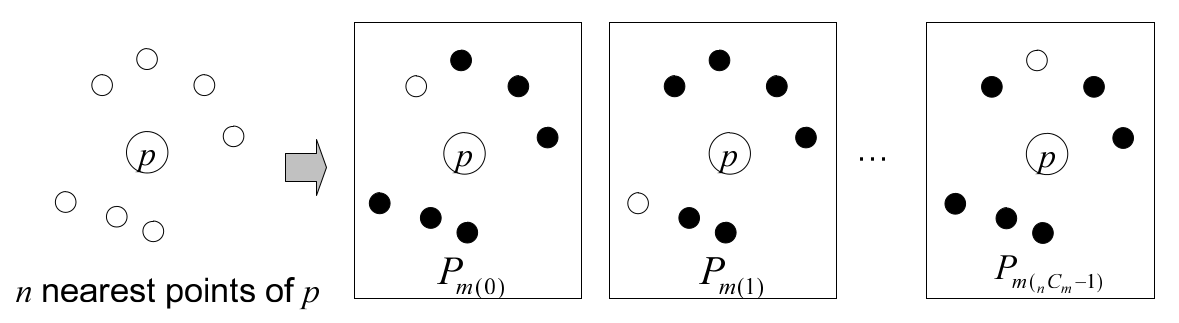
\includegraphics[width=0.9\textwidth]{nearestLLAH.png}
  \caption{LLAH: Todas la posibles combinaciones de \textit{m}(=6) puntos de los \textit{n}(=7) puntos contiguos a \textit{p} (Nakai y Kise)}
  \label{fig:nearest}
\end{figure}

\subsubsection{Almacenamiento y Recuperación}
En LLAH las imágenes se almacenan y recuperan mediante una tabla hash. En primer lugar se calculan y almacenan los descriptores de la imagen de forma preliminar. Cuando se da una imagen para recuperar, se calculan los descriptores de la consulta y se buscan y contabilizan los documentos posibles en los que coincidan el mismo descriptor. Finalmente, el documento que obtiene el mayor número de votos (descriptores encontrados)  es devuelto como resultado del proceso de recuperación


\subsection{Limitaciones en la identificación de documentos}
El análisis de documentos mediante cámaras tiene una serie de ventajas sobre aquellos que están basados en la adquisición mediante escáner. Las cámaras son pequeñas y fáciles de transportar. También se pueden utilizar en cualquier entorno y sobre documentos que por su formato sean difíciles de manipular en un escáner como periódicos, libros, o manuscritos antiguos. Incluso para capturar texto que no se encuentra en papel, como carteles en fachadas, o texto que se encuentre el objetos que se muevan por la escena.

En la mayoría de casos, los escáneres obtienen mejor calidad en la captura de calidad que las realizadas mediante cámaras, pero los sistemas basados en cámaras son mucho más flexibles y portables. 

\subsubsection{Problemática asociada}
Casi todos los algoritmos de reconocimiento de documentos obtienen grandes resultados partiendo de imágenes limpias, en alta resolución y con contrastes claramente definidos entre el texto y el fondo. Sin embargo, mediante la captura con cámaras debido a su naturaleza, a la forma en que se realiza la captura y el entorno en que nos encontremos se presentan una serie de dificultades que deben ser tenidas en cuenta.  
\begin{description}
\item[Baja resolución] Las imágenes obtenidas con las cámaras suelen estar en baja resolución, bien por las limitaciones del sensor, o por que la capacidad de computo del dispositivo que la contiene es limitada. Mientras que con un escáner es normal trabajas con una resolución de entre 150 a 600 dpi, el mismo texto en una captura con una cámara rodaría los 50 dpi.
\item[Iluminación no uniforme] La cámara, al contrario que el escáner no tiene control de la iluminación de la escena. En la captura mediante cámaras es normal encontrarse con iluminación no uniforme, varias fuentes de luz con temperaturas de color diferentes, sombras o reflejos que degradan la calidad de la imagen.
\item[Distorsión por perspectiva] Al capturar el texto sin estar la cámara paralela al plano en el que se encuentra el documento, se está produciendo una distorsión por perspectiva. Esto provoca que el texto presente distintos tamaños a lo largo de la imagen o que se produzca una deformación que impida el correcto reconocimiento de los caracteres. 
\item[Distorsión de la lente] Las cámara incorporadas a los teléfonos móviles suelen tener una distancia focal menor para obtener un mayor ángulo de visión. La consecuencia de esto es que la lente exagera la perspectiva de los objetos, provocando mayor distorsión en las líneas cuanto más cerca se encuentre la lente del objeto.
\item[Fondos complejos] El caso ideal para la extracción de texto es que el fondo sea totalmente uniforme y con contraste diferenciado. Una mala iluminación provocará alteraciones de tono y contraste entre texto y fondo, que dificultará la segmentación el texto. 
\item[Zoom y autoenfoque] Las cámaras actuales están equipadas con sistemas de zoom y autoenfoque. Una captura en la que existan distintos planos de profundidad o una mala iluminación provocará que el sistema de autoenfoque tenga dificultades para estabilizarse y durante ese tiempo las imágenes sean borrosas o fuera de foco.
\item[Objetos móviles] Por la propia naturaleza de los dispositivos móviles se entiende que o bien el dispositivo o el objeto a fotografiar está en movimiento (o incluso ambos). Si la velocidad de obturación de la cámara no es lo suficientemente rápida, la imagen obtenida estará movida.
\item[Ruido del sensor] Para compensar entornos con poca luz, las cámaras aumentan la sensibilidad amplificando la señal generada por las celdas del sensor. Como estos elementos tienen una emisión de señal de base mas o menos fija, al capturar una señal lumínica débil y amplificarla, estamos amplificando también una buena porción de la emisión de datos aleatoria, con lo que se mezclará una cantidad de señal aleatoria sin contenido a la señal correspondiente a la imagen. Cuanto mayor sea la amplificación, más ruido se va a generar y peor calidad de imagen vamos a obtener. 
\item[Compresión de imagen] Normalmente la imagen obtenida por el sensor se almacena comprimida mediante algoritmos con perdida de información como JPEG. La utilización de ratios altos de compresión provoca que se generen artefactos y distorsiones apreciables que restan nitidez a la imagen.
\item[Algoritmos ligeros] El objetivo final es integrar los algoritmos de análisis en los dispositivos móviles. Se deben implementar algoritmos computacionalmente eficientes ya que en la mayoría de los casos los recursos disponibles como memoria  y la capacidad de computo son limitadas.
\end{description}



% Local Variables:
%  coding: utf-8
%  mode: latex
%  mode: flyspell
%  ispell-local-dictionary: "castellano8"
% End:
